%%
%% This is file `example.tex',
%% generated with the docstrip utility.
%%
%% The original source files were:
%%
%% coppe.dtx  (with options: `example')
%% 
%% This is a sample monograph which illustrates the use of `coppe' document
%% class and `coppe-unsrt' BibTeX style.
%% 
%% \CheckSum{1648}
%% \CharacterTable
%%  {Upper-case    \A\B\C\D\E\F\G\H\I\J\K\L\M\N\O\P\Q\R\S\T\U\V\W\X\Y\Z
%%   Lower-case    \a\b\c\d\e\f\g\h\i\j\k\l\m\n\o\p\q\r\s\t\u\v\w\x\y\z
%%   Digits        \0\1\2\3\4\5\6\7\8\9
%%   Exclamation   \!     Double quote  \"     Hash (number) \#
%%   Dollar        \$     Percent       \%     Ampersand     \&
%%   Acute accent  \'     Left paren    \(     Right paren   \)
%%   Asterisk      \*     Plus          \+     Comma         \,
%%   Minus         \-     Point         \.     Solidus       \/
%%   Colon         \:     Semicolon     \;     Less than     \<
%%   Equals        \=     Greater than  \>     Question mark \?
%%   Commercial at \@     Left bracket  \[     Backslash     \\
%%   Right bracket \]     Circumflex    \^     Underscore    \_
%%   Grave accent  \`     Left brace    \{     Vertical bar  \|
%%   Right brace   \}     Tilde         \~}
%%
\documentclass[msc]{coppe}

\usepackage{booktabs}% tabelas mais bonitas
\usepackage{rotating}% rodando coisas, como tabelas
\usepackage{longtable} % tabelas longas
\usepackage[most]{tcolorbox} % caixas de texto
\usepackage{amsmath,amssymb}
\usepackage{hyperref}

\usepackage{multirow}
\usepackage{changepage} 

\usepackage{adjustbox} 

\usepackage{xcolor, colortbl} % For more complex coloring of cells
\usepackage{hhline} % For double lines

\usepackage{algorithm}
% \usepackage{algorithmic}
\usepackage{algpseudocode}

\makelosymbols
\makeloabbreviations

\begin{document}
  \title{Comparative Analysis of Single and Multi-Agent Large Language Model Architectures for Domain-Specific Tasks in Well Construction}
  \foreigntitle{Comparative Analysis of Single and Multi-Agent Large Language Model Architectures for Domain-Specific Tasks in Well Construction}
  \author{Vitor}{Brandão Sabbagh}
  \advisor{Prof.}{Geraldo}{Bonorino Xexéo}{D.Sc.}

  \examiner{Prof.}{Nome do Primeiro Examinador Sobrenome}{D.Sc.}
  \examiner{Prof.}{Nome do Segundo Examinador Sobrenome}{Ph.D.}
  \examiner{Prof.}{Nome do Terceiro Examinador Sobrenome}{D.Sc.}
  \examiner{Prof.}{Nome do Quarto Examinador Sobrenome}{Ph.D.}
  \examiner{Prof.}{Nome do Quinto Examinador Sobrenome}{Ph.D.}
  \department{PESC}
  \date{07}{2025}

  \keyword{Large Language Models}
  \keyword{Agentes}
  \keyword{Construção de Poços de Petroleo}

  \maketitle

  \frontmatter
  \dedication{Para Carolina, minha companheira de vida.}

  \chapter*{Agradecimentos}

    Gostaria de agradecer a todos. [família, amigos, etc]

    Estendo minha gratidão aos especialistas em engenharia de poços, Marcelo Grimberg, Rafael Peralta e Lorenzo Simonassi, cuja expertise e dedicação contribuíram significativamente para esta pesquisa.

    
  \begin{abstract}

    Apresenta-se, nesta tese, a aplicação de grandes modelos de linguagem (LLM) no setor de petróleo e gás, especificamente em tarefas de construção e manutenção de poços. O estudo avalia o desempenho de uma arquitetura baseada em LLM de agente único e de múltiplos agentes no processamento de diferentes tarefas, oferecendo uma perspectiva comparativa sobre sua precisão e as implicações de custo de sua implementação. Os resultados indicam que sistemas multiagentes oferecem desempenho melhorado em tarefas de perguntas e respostas, com uma medida de veracidade 28\% maior do que os sistemas de agente único, mas a um custo financeiro mais alto. Especificamente, a arquitetura multiagente incorre em custos que são, em média, 3,7 vezes maiores do que os da configuração de agente único, devido ao aumento do número de tokens processados. Por outro lado, os sistemas de agente único se destacam em tarefas de texto para SQL (Linguagem de Consulta Estruturada), especialmente ao usar o Transformador Pré-Treinado Generativo 4 (GPT-4), alcançando uma pontuação 15\% maior em comparação com as configurações multiagentes, sugerindo que arquiteturas mais simples podem, às vezes, superar a complexidade. A novidade deste trabalho reside em seu exame original dos desafios específicos apresentados pelos dados complexos, técnicos e não estruturados inerentes às operações de construção de poços, contribuindo para o planejamento estratégico da adoção de aplicações de IA generativa, fornecendo uma base para otimizar soluções contra parâmetros econômicos e tecnológicos.

  \end{abstract}

  \begin{foreignabstract}


    This article explores the application of large language models (LLM) in the oil and gas  sector, specifically within well construction and maintenance tasks. The study evaluates the performances of a single-agent and a multi-agent LLM-based architecture in processing different tasks, offering a comparative perspective on their accuracy and the cost implications of their implementation. The results indicate that multi-agent systems offer improved performance in question and answer tasks, with a truthfulness measure 28\% higher than single-agent systems, but at a higher financial cost. Specifically, the multi-agent architecture incurs costs that are, on average, 3.7 times higher than those of the single-agent setup due to the increased number of tokens processed. Conversely, single-agent systems excel in text-to-SQL (Structured Query Language) tasks, particularly when using Generative Pre-Trained Transformer 4 (GPT-4), achieving a 15\% higher score compared to multi-agent configurations, suggesting that simpler architectures can sometimes outpace complexity. The novelty of this work lies in its original examination of the specific challenges presented by the complex, technical, unstructured data inherent in well construction operations, contributing to strategic planning for adopting generative AI applications, providing a basis for optimizing solutions against economic and technological parameters. 

  \end{foreignabstract}

  \tableofcontents
  \listoffigures
  \listoftables
  \printlosymbols
  \printloabbreviations

  \mainmatter
  \chapter{Introdução}

          % Segundo a norma de formatação de teses e dissertações do
          % Instituto Alberto Luiz Coimbra de Pós-graduação e Pesquisa de
          % Engenharia (COPPE), toda abreviatura deve ser definida antes de
          % utilizada.\abbrev{COPPE}{Instituto Alberto Luiz Coimbra de Pós-gradua{\c
          % c}\~ao e Pesquisa de Engenharia}.
        
          % Do mesmo modo, é imprescindível definir os símbolos, tal como o
          % conjunto dos números reais $\mathbb{R}$ e o conjunto vazio $\emptyset$.
          % \symbl{$\mathbb{R}$}{Conjunto dos números reais}
          % \symbl{$\emptyset$}{Conjunto vazio}
        
          % Para as listas de abreviaturas e símbolos funcionarem, é necessário rodar o \verb|latexmkrc|. O Overleaf faz isso automaticamente. Caso haja um problema, verifique se o arquivo \verb|coppe.ist| está no diretório. Também é útil compilar do início e apagar todos os arquivos desnecessários.
    
        
    \section{Contextualização}
        
        % [IA-GEN NA INDÚSTRIA]
        Na dinâmica em constante mudança da indústria de petróleo e gás (O\&G), a transformação digital emergiu como um elemento chave para alcançar eficiência operacional, sustentabilidade e competitividade.
        Na vanguarda dessa transformação estão os Modelos de Linguagem de Grande Escala (LLMs), que têm o potencial de processar consultas não estruturadas, mapear alternativas e aconselhar os usuários sobre possíveis ações \cite{Kar2023}.
        Também observamos a vantagem do aumento do engajamento, cooperação, acessibilidade e, em última análise, lucratividade.
        Esses modelos redefinem paradigmas em gestão do conhecimento e recuperação de informações e impactam uma variedade de outras áreas \cite{Eckroth2023}, tornando crucial a adoção dessas tecnologias para permanecer competitivo.
        
        % [ESTUDO AUMENTO PRODUTIVIDADE]
        Um estudo conduzido por \cite{Dellacqua2023}, em colaboração com o Boston Consulting Group, demonstra que em tarefas intensivas em conhecimento, consultores equipados com acesso a LLMs como o GPT-4 não apenas completaram as tarefas mais eficientemente (25,1\% mais rapidamente em média), mas também com qualidade substancialmente maior, alcançando resultados mais de 40\% melhores em comparação com aqueles sem assistência de IA \cite{Dellacqua2023}. O aumento da produtividade dos trabalhadores do conhecimento foi de 12\% em média.
        Para ilustrar, se considerarmos os \$2,8 bilhões gastos em remuneração por uma grande empresa de petróleo, dos quais 60\% vão para trabalhadores do conhecimento (\$1,6 bilhões), um aumento de 12\% na produtividade poderia ser visto como gerando um valor adicional de \$204 milhões em produção da mesma força de trabalho.
        % [AUMENTO DO PIB DEVIDO A GEN AI]
        Indicadores econômicos mais amplos preveem transformações significativas devido à IA generativa (Gen-AI) em vários setores.
        Um relatório do Goldman Sachs \cite{Hatzius2023} destaca que a Gen-AI está prestes a aumentar o PIB global em quase 7\%, aumentando o crescimento da produtividade em 1,5 pontos percentuais na próxima década.

    \section{Motivação}
        % [PROBLEMA DE DADOS NA INDÚSTRIA EM GERAL]
        Expandindo a discussão mais ampla sobre a utilização de dados nas organizações, um problema importante é o desafio de extrair informações relevantes de extensas bases de dados \cite{Singh2023}.
        Inicialmente, o desafio de conhecer, encontrar e acessar dados representa um obstáculo significativo para os processos de tomada de decisão. Colaboradores em empresas de O\&G frequentemente enfrentam a tarefa intensiva de buscar manualmente em grandes repositórios de dados para encontrar informações úteis.
        
        % [PROBLEMA DE DADOS NO O&G]
        Focando especificamente nas atividades de perfuração e completação de poços offshore e onshore, um grande desafio reside na natureza inerentemente complexa e técnica dos dados envolvidos, que podem ser de vários tipos: operações, projetos, tecnologias, cadeias de suprimentos e outros.
        A ineficiência em aproveitar grandes volumes de dados não estruturados agrava esses desafios, como observado por \cite{Singh2023}. Uma quantidade significativa dos dados gerados e coletados neste setor é não estruturada, variando de relatórios de texto e e-mails a imagens e vídeos de atividades de exploração e produção.
        As empresas de O\&G enfrentam desafios na extração de informações relevantes de vastos dados não estruturados, impactando a tomada de decisões e a inovação \cite{Singh2023}.
        Exemplos incluem centenas de relatórios operacionais diários de sondas de perfuração, projetos de execução de poços, relatórios de tempo não produtivo (NPT) e documentos de lições operacionais aprendidas, conforme ilustrado na Figura \ref{fig:report_example}.
        Como resultado, informações valiosas podem permanecer inexploradas e o potencial para encontrar insights, tomar decisões informadas e inovar é significativamente comprometido.
        \cite{Singh2023} destaca as capacidades e o potencial de chatbots habilitados por IA Generativa para o setor de O\&G, particularmente em melhorar a análise de perfuração e produção para alcançar melhores resultados de negócios. O autor conclui que as empresas que adotarem essas tecnologias nos próximos anos verão vantagens claras.
        
        \begin{figure}[t]
            \centering
            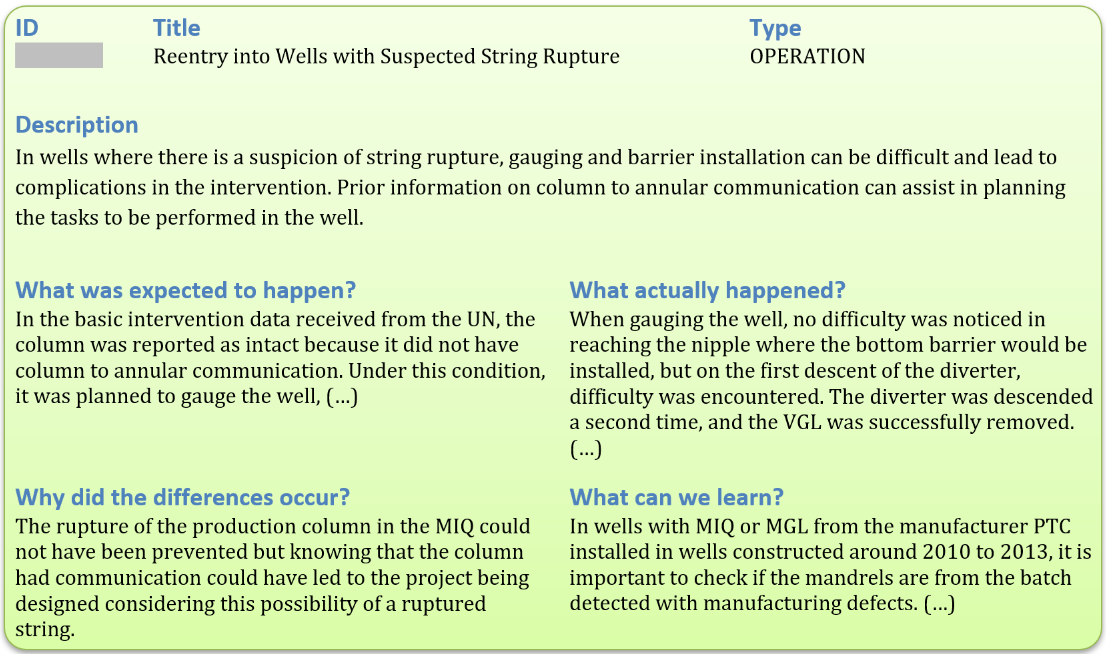
\includegraphics[width=1\textwidth]{images/report_example.png}
            \caption{Amostra de lição aprendida de perfuração e completação. Documento parcial de uma grande empresa de petróleo. (traduzido do português)}
            \label{fig:report_example}
        \end{figure}
        
        A implantação de tecnologias de IA enfrenta desafios como dados tendenciosos, alucinações e falta de explicabilidade \cite{Hadi2023}, necessitando de uma abordagem equilibrada. Embora pesquisas anteriores tenham abordado amplamente a IA na indústria, este estudo examina de forma única os desafios e soluções para dados não estruturados complexos em operações de O\&G. Este trabalho aborda a lacuna na compreensão do desempenho de arquiteturas LLM de agente único versus multi-agente em tarefas específicas de domínio, como engenharia de poços, oferecendo insights sobre sua eficácia e relação custo-benefício. A adoção de LLM por uma grande empresa de petróleo destaca o potencial dessas tecnologias para transformar a análise e gestão de dados.
    
    \section{Objetivos}
    
        Esta pesquisa aborda diretamente os desafios enfrentados por grandes empresas de petróleo. Ao investigar as vantagens comparativas e limitações de várias arquiteturas de IA generativa (Gen-AI), incluindo sistemas de agente único e multiagente, este estudo visa identificar as soluções mais eficientes e econômicas.
        Os objetivos específicos desta pesquisa são avaliar a adequação e eficácia dos sistemas multiagentes baseados em LLMs para tarefas complexas e específicas de domínios na engenharia de poço, com o objetivo de otimizar o acesso à informação e a tomada de decisões.
        O estudo compara sistemas de IA de agente único e multiagente em termos de sua capacidade de responder a consultas relacionadas à engenharia de poços. Ele também mapeia os possíveis obstáculos e limitações associados à implantação de aplicações de Gen-AI.
        
        Os insights obtidos com esta pesquisa visam contribuir diretamente para os objetivos estratégicos das empresas de O\&G, melhorando o acesso a informações sobre engenharia de poços e tarefas de análise de dados automatizadas.
        Uma compreensão abrangente dos desafios e limitações associados à Gen-AI permitirá decisões informadas sobre sua adoção, maximizando o retorno sobre o investimento.
        
    \section{Delimitação do Escopo de Negócio}
        
        Para contextualizar o escopo deste estudo, é necessário entender o ciclo de vida de um campo de petróleo, que começa com a Exploração, progride para o Desenvolvimento da Produção, segue com a produção efetiva e culmina no descomissionamento \cite{Badiru2016}. A construção de poços, que envolve a perfuração e completação de poços para extração de hidrocarbonetos, é uma atividade dentro da fase de Desenvolvimento da Produção \cite{Thomas2004}. A Gen-AI tem o potencial de impactar cada uma dessas fases, mas o foco deste trabalho está nas operações das fases de desenvolvimento e manutenção.
        
        A construção de poços é uma atividade altamente especializada que envolve a perfuração e completação de poços para extração de hidrocarbonetos \cite{Thomas2004}. Neste contexto, a Gen-AI pode ser aplicada de várias maneiras. Por exemplo, um chatbot pode gerenciar o conhecimento respondendo a perguntas sobre operações e projetos de poços, recuperando informações dos bancos de dados da organização. Além disso, agentes baseados em LLMs podem ser usados em revisões executivas de projetos para garantir que as operações de perfuração ou completação estejam em conformidade com os padrões da organização e aderem às melhores práticas operacionais. Ademais, a Gen-AI pode realizar inferências em bancos de dados não estruturados para extrair informações específicas de relatórios de texto e obter dados estruturados.
     
    \section{Estrutura da Dissertação}

        ****SERÁ FEITO POR ÚLTIMO****


    
\chapter{Revisão de Literatura} 

    \section{IA na indústria de petroleo}
    
        O uso de IA na indústria de Exploração e Produção (E\&P) de petróleo tem sido extenso. Nas últimas décadas, a maioria das aplicações de IA na indústria envolve mineração de dados e redes neurais \cite{Bravo2014}. Um exemplo é o trabalho de \cite{Gudala2021} sobre a otimização das propriedades de fluxo de óleo pesado, utilizando redes neurais para otimizar parâmetros que influenciam o fluxo.
        
        Uma contribuição significativa vem da integração do conhecimento do domínio com estruturas digitais para aprimorar a tomada de decisões em tratamentos de fraturamento. Essa abordagem, demonstrada por \cite{Khan2024}, utiliza aprendizado de máquina para melhorar a eficiência operacional e reduzir custos.
        
        Outro desenvolvimento foi um fluxo de trabalho de aprendizado profundo proposto por \cite{Gohari2024}, com a geração de logs gráficos sintéticos de poços através da aplicação de aprendizado por transferência. Esses desenvolvimentos ilustram o potencial da IA em melhorar processos e a precisão e eficiência da análise de dados \cite{Rahmani2021}.
        
        Processamento de Linguagem Natural (PLN) situa-se na interseção da ciência da computação e linguística, representando um domínio dentro da inteligência artificial que visa permitir que computadores compreendam e processem a linguagem humana de maneira significativa e eficaz \cite{Liddy2001}. Este campo integra uma variedade de técnicas computacionais para analisar e representar texto em vários níveis de detalhe linguístico, buscando emular a compreensão da linguagem humana. Como uma área ativa de pesquisa, tradicionalmente o PLN emprega múltiplas camadas de análise linguística, cada uma contribuindo de forma única para a interpretação e geração de linguagem, encontrando aplicações práticas em diversos setores \cite{Liddy2001}.
        
        Na indústria de O\&G, a gestão de dados não estruturados, como textos, imagens e documentos, é crucial, com o Processamento de Linguagem Natural (PLN) e o Aprendizado de Máquina desempenhando papéis chave. Pesquisas de \cite{Antoniak2016} e \cite{Castineira2018} exploraram o uso de PLN para analisar riscos e relatórios de perfuração.
    
        \section{Modelos de Linguagem de Grande Escala (LLMs).}  
        
            Os LLMs são modelos avançados baseados em redes neurais projetados para entender e gerar textos semelhantes aos humanos. Eles utilizam a arquitetura Transformer, apresentada no artigo seminal "Attention is All You Need" por \cite{Vaswani2017}. Esta arquitetura depende de mecanismos de auto-atenção, permitindo que o modelo avalie efetivamente a importância de diferentes palavras em uma sentença.
            
            O surgimento dos LLMs tornou possível compreender e produzir informações textuais. Espera-se que esses sistemas revolucionem várias indústrias ao apoiar processos complexos de tomada de decisão. Os modelos GPT \cite{OpenAI2023}, em particular, aproveitam seu vasto conjunto de dados de treinamento para fornecer respostas semelhantes às humanas \cite{Mosser2024}, o que pode ser altamente benéfico em contextos que exigem compreensão e geração de linguagem natural.
            
            Como destacado por \cite{Singh2023}, a integração de soluções baseadas em LLMs, como chatbots conversacionais, oferece uma abordagem para otimizar operações em vários segmentos de negócios, incluindo perfuração, completação e produção. \cite{Singh2023} usa modelos LLMs para extrair, analisar e interpretar conjuntos de dados, permitindo a geração de insights e recomendações.
            
            Apesar de seu impacto generalizado, os modelos de linguagem não estão isentos de limitações. Em muitas aplicações específicas da indústria, as informações críticas necessárias são frequentemente proprietárias, não compartilhadas com terceiros e, portanto, ausentes dos dados de treinamento desses LLMs \cite{Mosser2024}. Essa lacuna significa que os modelos GPT podem não ter acesso às informações mais atualizadas ou sensíveis necessárias para certas tarefas. Além disso, devido à sua natureza probabilística, os LLMs podem experimentar alucinações, produzindo respostas confiantes, mas incorretas ou sem sentido, com base na entrada do usuário \cite{OpenAI2023}.
    
    
        \section{Tarefas de Pergunta e Resposta (Q\&A).}
        
            A tarefa de Pergunta e Resposta (Q\&A) representa um método para facilitar a transferência de conhecimento entre indivíduos dentro das organizações \cite{Iske2005}. Conceitualmente, os sistemas Q\&A são projetados para conectar indivíduos que possuem conhecimento específico com aqueles que buscam esse conhecimento por meio de um formato estruturado de pergunta e resposta.
            O papel do Q\&A no cenário da documentação, exemplificado por plataformas como o Stack Overflow, destaca sua importância em disciplinas técnicas \cite{Treude2011}. Esse entendimento pode orientar as organizações a tomarem decisões mais informadas sobre a implementação de tais sistemas para aprimorar a transferência de conhecimento e o aprendizado organizacional \cite{Iske2005}.
    
    
        \section{Tarefas Text-to-SQL}
        
            As tarefas de Text-to-SQL no contexto da inteligência artificial envolvem a tradução automática de perguntas ou comandos em linguagem natural para consultas SQL (Structured Query Language) estruturadas \cite{Qin2022}. Esta é uma área importante no processamento de linguagem natural (NLP), permitindo que os usuários interajam com bancos de dados usando linguagem comum, em vez de precisar saber como escrever consultas SQL complexas.
            
            A chegada de modelos de linguagem avançados como GPT-3 e GPT-4 \cite{OpenAI2023} marcou um salto significativo nas aplicações de Text-to-SQL \cite{Singh2023}, demonstrando capacidades notáveis no tratamento dessas tarefas. Isso pode ser atribuído ao seu extenso treinamento em conjuntos de dados diversificados \cite{Deng2021}, que incluem não apenas grandes volumes de texto, mas também dados estruturados como tabelas e código, permitindo ao modelo entender as relações intrincadas entre linguagem e estruturas de dados. O estudo de \cite{Deng2023} introduz um framework de pré-treinamento para tradução de texto para SQL, enfatizando o alinhamento entre texto e tabelas nas tarefas de Text-to-SQL.
        
        
        \section{Multi-Agent Setup} 
    
            Conforme demonstrado por \cite{xi2023rise}, a busca pela Inteligência Artificial Geral (AGI) tem se beneficiado significativamente do desenvolvimento de agentes baseados em LLM, capazes de percepção, tomada de decisão e ação em diversos cenários.        
            Seu estudo delineia uma estrutura fundamental para tais agentes, composta por componentes de cérebro, percepção e ação, que podem ser personalizados para várias aplicações, incluindo cenários de agente único, sistemas multi-agentes e colaboração humano-agente. 
            A pesquisa abrangente destaca o papel crucial dos LLMs no avanço em direção à AGI, sugerindo um horizonte promissor para a eficiência operacional e os processos de tomada de decisão em configurações organizacionais complexas \cite{xi2023rise}.
            \cite{Li2024} demonstrou que, através de um método de amostragem e votação, o desempenho dos LLMs escala com o número de agentes instanciados.
            Outro framework de código aberto é o AutoGen \cite{Wu2023}, que permite a criação de aplicações multi-agentes LLM, possibilitando a personalização em vários modos. Ele apoia diversas aplicações em campos como matemática, programação e pesquisa operacional, demonstrando sua eficácia por meio de estudos empíricos \cite{Wu2023}.




\chapter{Introdução 2 [CANCELADO]} 


    \section{Contextualização 2 [ok]}

        % The oil and gas industry is currently navigating a complex landscape characterized by significant challenges in well construction and maintenance. These challenges include managing vast amounts of data, ensuring operational efficiency, and maintaining safety standards. The integration of advanced technologies such as Large Language Models (LLMs) offers promising solutions to optimize processes and enhance decision-making in this sector. LLMs, with their ability to process and analyze large datasets, can significantly improve the efficiency and accuracy of well construction and maintenance operations. This section will explore the current challenges in the oil and gas industry, particularly in well construction, and introduce the potential of LLMs as transformative tools in this domain.
        
        ****USAR O ANTERIOR****

        
        \subsection{Challenges in Well Construction and Maintenance}
        
            % Data Management: 
            The oil and gas industry generates substantial volumes of data from various sources, including sensor data, reports, and historical records. However, much of this data remains underutilized due to difficulties in retrieval and analysis, leading to inefficiencies in well construction and maintenance operations \cite{Michael_Yi_2024}; \cite{Myriam_Amour_2024}.
            
            % Operational Efficiency: 
            The need for real-time decision-making in well construction is critical. Traditional methods often fall short in providing timely insights, which can lead to increased downtime and higher operational costs \cite{E_Ferrigno_2024}.
            
            % Safety and Environmental Concerns: 
            Ensuring safety and minimizing environmental impact are paramount in well construction. The complexity of operations necessitates robust data governance and standardization to maintain safety standards and comply with regulations \cite{Syatria_Kumala_Putra_2024}.
            Potential of LLMs in Optimizing Processes
            
        \subsection{Potential of LLMs in Optimizing Well Construction}
               
            % Enhanced Data Retrieval and Analysis: 
            LLMs can significantly improve the retrieval and analysis of well construction data by providing quick access to relevant information and facilitating complex data queries. This capability reduces the time required for data processing and enhances decision-making efficiency \cite{Michael_Yi_2024}; \cite{Myriam_Amour_2024}.
            
            % Real-Time Decision Support: 
            By integrating LLMs into drilling control rooms, companies can achieve real-time classification and analysis of data, which is crucial for responding to critical events during drilling operations. This integration has been shown to enhance decision-making efficiency by over 50 times \cite{E_Ferrigno_2024}.
            
            % Domain-Specific Knowledge Integration: 
            LLMs empowered by domain-specific knowledge bases (LLM-DSKB) can provide more accurate and relevant insights for industrial applications, addressing the limitations of general LLMs in handling technical issues specific to the oil and gas sector \cite{Huan_Wang_2023}.
            
            
            % Broader Perspective on LLMs in the Industry
        \subsection{Broader Perspective on LLMs in the Industry}
        
            While LLMs offer significant potential to optimize well construction and maintenance processes, their implementation is not without challenges. The integration of LLMs requires careful consideration of data quality and infrastructure to ensure reliable and accurate outputs. Additionally, the lack of domain-specific expertise in existing LLMs can limit their effectiveness in technical applications, necessitating the development of specialized knowledge bases to enhance their utility . Furthermore, the adoption of LLMs in the oil and gas industry must be balanced with considerations of cost, scalability, and the need for ongoing collaboration between industry experts and AI developers to fully realize their potential .
        
        
        % \subsection{aaaaa}
        % \subsection{aaaaa}
        % \subsection{aaaaa}

    \section{Motivação 2 [scispace]}

        [[[[ SCISPACE ]]]]
        PESQUISAR SOBRE DESAFIOS E MOTIVAÇÕES PARA USO DE AGENTES E MULTI-AGENTES (EM DOMÍNIOS ESPECIFICOS?)

    \section{Contribuições 2 [final]}
    
        ****SERÁ FEITO POR ÚLTIMO****
        
    \section{Objetivo do trabalho 2 [final]}

        ****SERÁ FEITO POR ÚLTIMO****

    \section{Organização do trabalho 2 [final]}

        ****SERÁ FEITO POR ÚLTIMO****

    

\chapter{Revisão 2 [CANCELADO]} 


    \section{Large Language Models}


    \section{aaaaa}


    \section{aaaaa}


    \section{aaaaa}






\chapter{Experimento 1}
    

    \section{Metodologia}
        
        Esta seção descreve a abordagem e as ferramentas empregadas para investigar a eficácia de um agente baseado em modelo de linguagem em responder a consultas específicas no domínio da construção e manutenção de poços. Primeiramente, a preparação, seleção e utilização das fontes de dados são descritas, explicando como cada uma contribui para a base de conhecimento da qual o agente deriva suas respostas.
            
        \subsection{Preparação de Dados}
            
            Este experimento foi conduzido no departamento de construção de poços de uma grande empresa de petróleo. A escolha das tarefas foi focada em gestão de conhecimento técnico e análise de dados. Exemplos de consultas utilizadas no experimento estão listados na Tabela~\ref{table:question_examples}. As fontes de dados para a execução dessas tarefas foram escolhidas para cobrir uma variedade de cenários operacionais na atividade de construção e manutenção de poços: Itens de Conhecimento Operacional, NPTs Operacionais (Tempo Não Produtivo) e um Localizador de Colaboradores.
    
    
            \begin{table}[ht]
                \centering % Centraliza a tabela
                \caption{Exemplo de Tabela de Números}
                \label{tab:exemplo_numeros}
                \begin{tabular}{ccc} % Define a quantidade de colunas
                    \toprule % Linha superior
                    \textbf{Coluna 1} & \textbf{Coluna 2} & \textbf{Coluna 3} \\ % Cabeçalhos
                    \midrule % Linha média
                    1 & 2 & 3 \\ % Primeira linha de dados
                    4 & 5 & 6 \\ % Segunda linha de dados
                    7 & 8 & 9 \\ % Terceira linha de dados
                    10 & 11 & 12 \\ % Quarta linha de dados
                    \bottomrule % Linha inferior
                \end{tabular}
            \end{table}
    
            
            \begin{table}[h]
                \centering
                \caption{Exemplos de consultas usados neste estudo. }
                \begin{tabular}{l l }
                    \toprule % Linha superior
                    \textbf{Categoria} & \textbf{Exemplo de Consulta} \\ 
                    \midrule % Linha média
                    Q\&A & Como a presença de sílica na composição da pasta de cimento \\
                         & \quad afeta sua estabilidade térmica a altas temperaturas? \\ 
                         & Quais são os principais desafios e riscos associados\\
                         &  \quad ao tamponamento e abandono através da tubulação em\\
                         &  \quad poços altamente desviados? \\ 
            
                         & O que pode causar a formação de hidratos no conector da\\ 
                         & \quad Ferramenta de Corrida de Árvore durante a lavagem da\\ 
                         & \quad mangueira HCR (Alta Resistência ao Colapso) antes de\\ 
                         & \quad conectar à Árvore de Natal Molhada? \\ 
                         & O que pode causar a válvula de segurança do fundo do poço\\ 
                         & \quad  permanecer aberta devido à formação de hidratos nas\\ 
                         & \quad  linhas de controle? \\ 
                         & O que pode causar danos aos protetores de rosca e áreas de\\ 
                         & \quad  vedação das extremidades dos tubos armazenados no\\ 
                         & \quad  pátio de revestimento? \\ 
                         & O que pode causar alto arrasto e torque fora do fundo durante\\ 
                         & \quad  a perfuração de um poço com alta inclinação? \\ 
                         & Quais precauções devem ser tomadas ao realizar uma verificação\\ 
                         & \quad  superior do tampão de abandono em poços com maior inclinação? \\ 
                         & Quais são os fatores críticos a serem considerados ao escolher\\ 
                         & \quad  um fluido base para fabricar um tampão de suporte viscoso? \\ 
                         & Quais são as melhores práticas para gerenciar os parâmetros\\ 
                         & \quad  de perfuração durante o corte de cimento para evitar\\ 
                         & \quad  desgaste prematuro da broca? \\ 
            
                    Text-to-SQL & Qual foi o NPT de maior duração na sonda número 05? \\ 
                         & Quantos NPTs ocorreram na sonda número 06 durante agosto de\\ 
                         & \quad  2023? \\ 
                \bottomrule % Linha inferior        
                \end{tabular}
                \label{table:question_examples}
            \end{table}
    
            
                
            \emph{Itens de Conhecimento Operacional} Durante intervenções de perfuração, completação e workover, documentos chamados Itens de Conhecimento são escritos por especialistas, conforme ilustrado na Fig~\ref{fig:report_example}. Esses documentos podem ser de 4 tipos: Alerta Técnico, Lição Aprendida, Boa Prática e Observação de Poço. Esta é uma ferramenta para gestão do conhecimento, considerando o grande número e variedade de especialistas envolvidos e operações de poço realizadas.
            
            \emph{NPTs Operacionais (Tempo Não Produtivo)} A segunda fonte de dados refere-se a dados sobre anomalias ocorridas durante intervenções em poços, contendo informações como título, descrição do evento, poço onde ocorreu, tipo de operação, setor responsável, sonda envolvida, tempo perdido em horas, e datas de início e término do evento. Esses dados são críticos para a indústria, pois os NPTs representam períodos em que a operação de perfuração, completação ou manutenção é interrompida devido a algum problema técnico ou logístico. A identificação e análise desses eventos são essenciais para a melhoria contínua do processo, redução de custos e aumento da eficiência operacional. Ao entender as causas e circunstâncias desses incidentes, as organizações podem desenvolver estratégias para preveni-los no futuro, otimizando o tempo de operação.
            
            \emph{Localizador de Colaboradores} A terceira fonte de dados utilizada no experimento é um localizador de colaboradores, uma ferramenta importante dentro de uma organização para consultar e gerenciar dados de funcionários. Este sistema permite a busca rápida e identificação de colaboradores através de informações como nome, local de trabalho, empresa, matrícula e função. A importância dessa ferramenta para o experimento reside na possibilidade de cruzar dados de funcionários com outras fontes de informação para uma resposta mais completa pelo agente.
            
            Cada uma dessas fontes fornece insumos para que o agente ofereça uma visão mais precisa e atualizada das operações e da estrutura organizacional. Um conjunto de documentos e registros foi selecionado aleatoriamente de cada banco de dados, sobre os quais foram formuladas perguntas. Para cada documento, foram geradas até 3 perguntas, resultando em um conjunto de tarefas do tipo Q\&A e Text-to-SQL. Alguns exemplos são descritos na Tabela \ref{table:question_examples}.
    
    
    
            Neste trabalho, um agente baseado em metas \cite{Russell2020} foi implementado com o objetivo de responder com precisão a várias consultas. O agente opera em um ambiente equipado com múltiplas ferramentas para operações específicas de tarefas, como mostrado na Figura~\ref{fig:agent_environment}, e interage com os usuários para receber consultas.
            
            \begin{figure}[ht]
                \centering
                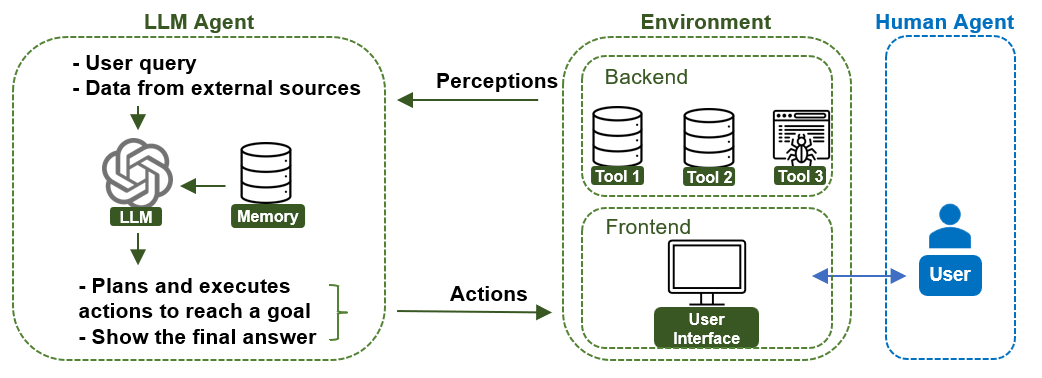
\includegraphics[width=1\textwidth]{images/agent_environment_4.png}
                \caption{Esquemático do agente baseado em LLM interagindo com um ambiente contendo ferramentas para operações específicas de tarefas, e a interface do Agente Humano para interação e feedback do usuário.}
                \label{fig:agent_environment}
            \end{figure}           
            
            Inicialmente, uma configuração de agentes foi implementada conforme descrito na Figura~\ref{fig:agent_config_1} usando o Framework AutoGen \cite{Wu2023} com uma arquitetura que permite a recuperação de informações e interação com o usuário. Este sistema consiste em:
            
            \begin{itemize}        
            
                \item \textbf{User Proxy:} representa a interface com o usuário e com ferramentas para acessar bancos de dados externos. A natureza modular das ferramentas permite que o User Proxy seja personalizado e expandido com base na variedade de fontes de dados e nos requisitos específicos do domínio de aplicação.
            
                \item \textbf{Agente:} alimentado por LLMs como GPT-4 e GPT-3, é o motor analítico do sistema. Este agente interpreta as consultas recebidas do User Proxy e formula respostas.
                                         
            \end{itemize}
            
            \begin{figure}[hbt]
                \centering
                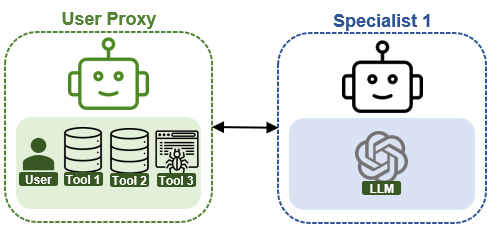
\includegraphics[width=.5\textwidth]{images/agent_config_1.png}
                \caption{Configuração do chat com um User Proxy \cite{Wu2023} e um Assistente.}
                \label{fig:agent_config_1}
            \end{figure}
            
            Para cada pergunta no conjunto de dados, o processo de tomada de decisão do agente é executado conforme descrito na Figura~\ref{fig:diagrama_agente_1}, inicialmente selecionando a ferramenta apropriada para responder a uma consulta e, finalmente, compilando as informações recuperadas para fornecer uma resposta final.
            
            \begin{figure}[h]
                \centering
                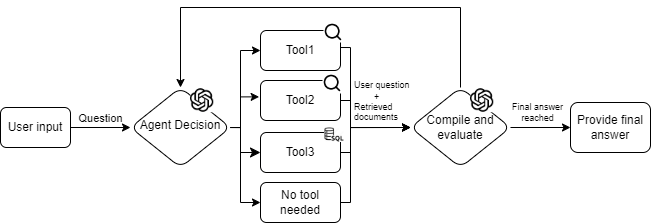
\includegraphics[width=1\textwidth]{images/agent_diagram_1.png}
                \caption{Processo de decisão do agente.}
                \label{fig:diagrama_agente_1}
            \end{figure}
    
    
    
            
            Neste experimento, três ferramentas foram consideradas no processo de tomada de decisão:
            
            \begin{itemize}
            
                \item \textbf{Ferramenta 1 - Pesquisa de Itens de Conhecimento:} uma ferramenta para pesquisar lições aprendidas que podem ser relevantes para a consulta.
                
            
                \item \textbf{Ferramenta 2 - Pesquisa de Colaboradores:} funcionalidade que permite a busca de informações relacionadas aos colaboradores de uma organização.
            
                \item  \textbf{Ferramenta 3 - Consulta SQL NPT:} interface para execução de consultas SQL em um banco de dados de NPTs operacionais. 
            
            \end{itemize}
            
            Paralelamente, há um caminho que permite ao Agente LLM fornecer uma resposta direta, sem a necessidade de recorrer a outras ferramentas, presumivelmente usado quando o agente já possui as informações necessárias. Finalmente, o agente apresenta a resposta final ao usuário, que é o produto de um processamento de modelo de linguagem, tomando como entradas a consulta do usuário e informações relevantes recuperadas e incluídas no contexto do prompt.
            
            A Tabela \ref{tab:tabela_inputs} fornece uma análise detalhada do desempenho e precisão de diferentes modelos, especificamente GPT-3.5-turbo e GPT-4, quando consultados sobre o impacto da sílica na estabilidade térmica da pasta de cimento em altas temperaturas. A tabela compara configurações de agente único e multiagentes, avaliando as saídas finais com base na veracidade, desempenho e comentários de especialistas. Para cada consulta, a tabela destaca a relevância e precisão das informações fornecidas pelos modelos, incluindo quaisquer seções extraviadas ou não relacionadas observadas pelos especialistas. Esta comparação abrangente permite uma avaliação aprofundada das capacidades dos modelos em gerar respostas precisas e relevantes para perguntas técnicas.
            
    
            \begin{adjustwidth}{-2cm}{-2cm} % Reduz a margem esquerda em 2cm 
            \begin{table}[ht] 
            \centering 
            \caption{Amostra de consulta com entradas, saídas e avaliações.} 
            \label{tab:tabela_inputs} 
            \footnotesize 
            \begin{tabular}{p{2cm}p{1cm}p{1cm}p{6cm}p{1.3cm}p{1.2cm}p{2cm}} 
            \toprule 
            \textbf{Consulta} & \textbf{Modelo} & \textbf{Config.} & \textbf{Saída} & \textbf{Veraci-\newline dade} & \textbf{Desem-\newline penho} & \textbf{Comentários} \\ 
            \midrule 
            \multirow{4}{=}{Como a presença de sílica na composição da pasta de cimento afeta sua estabilidade térmica em altas temperaturas?} & 
            \multirow{2}{=}{GPT-3.5-turbo} & 
            Agente único & 
            A presença de sílica na composição da pasta de cimento pode afetar sua estabilidade térmica em altas temperaturas devido a algumas características da sílica. A sílica é um material inorgânico que possui uma estrutura cristalina estável em altas temperaturas. Quando exposta a altas temperaturas, a sílica presente na pasta de cimento pode sofrer transformações estruturais, resultando em mudanças nas propriedades da pasta. [...] & 
            4 & 
            5 & 
            Criou uma seção que é irrelevante para a questão: "Além disso, a presença de sílica na composição da pasta de cimento pode afetar a resistência térmica do material. [...]" \\ 
            \cmidrule{3-7} 
             & & Multiagente & A presença de sílica na composição da pasta de cimento tem um efeito positivo na estabilidade térmica em altas temperaturas. A sílica é adicionada ao cimento para mitigar a retrogressão da resistência do cimento quando exposto a temperaturas acima de 230°F (110°C). Poços profundos ou aqueles com alto gradiente geotérmico podem exigir o uso de cimento com sílica para garantir a estabilidade térmica da pasta. [...] & 2 & 2 & Recuperou uma Lições Aprendidas não relacionada ao assunto (sobre plugs). \\ 
            \cmidrule{2-7} 
             & \multirow{2}{=}{GPT-4} & Agente único & A presença de sílica na composição da pasta de cimento aumenta a estabilidade térmica, especialmente em altas temperaturas. A sílica é usada para transformar o cimento em um material refratário, capaz de suportar condições extremas. [...] & 3 & 4 & Embora seja verdade, o item ao lado não é relevante para a questão: "No entanto, é importante notar que [...]." \\ 
            \cmidrule{3-7} 
             & & Multiagente & A sílica é adicionada ao cimento em uma proporção de 35\% em peso de cimento para mitigar a retrogressão (perda de resistência à compressão) do cimento no poço quando submetido a temperaturas acima de 230ºF (110ºC). [...] & 5 & 4 & Citou uma Lições Aprendidas não relacionada (mas verdadeira) sobre plugs, Lições Aprendidas LA7005. \\ 
            \bottomrule 
            \end{tabular} 
            \end{table}         
            \end{adjustwidth} 
    
    
            \subsection{Arquitetura Multi-Agente}        
            
                Uma segunda arquitetura que emprega múltiplos agentes foi implementada, cada um tendo uma ferramenta distinta para interagir com fontes de dados externas, como ilustrado na Figura \ref{fig:agent_config_2}. 
                Esta arquitetura também começa com a entrada do usuário. No entanto, como representado na Figura \ref{fig:diagrama_agente_MultiAgente_2}, o subsequente processo de 'Seleção de Palestrante' determina o agente especializado avaliado como mais adequado para responder à pergunta do usuário.            
                
                Quando uma consulta se enquadra no conhecimento direto do LLM, o caminho 'Nenhuma ferramenta necessária' é selecionado, e o agente correspondente responde sem o engajamento de outras ferramentas.
                O agente selecionado então 'Compila e avalia' as informações coletadas no contexto da consulta do usuário, garantindo uma resposta que seja tanto precisa quanto contextualizada. A etapa final, 'Fornecer resposta final', é onde o sistema multi-agente converge para entregar a resposta final e coerente ao usuário.
                    
                \begin{figure}[h]
                    \centering
                    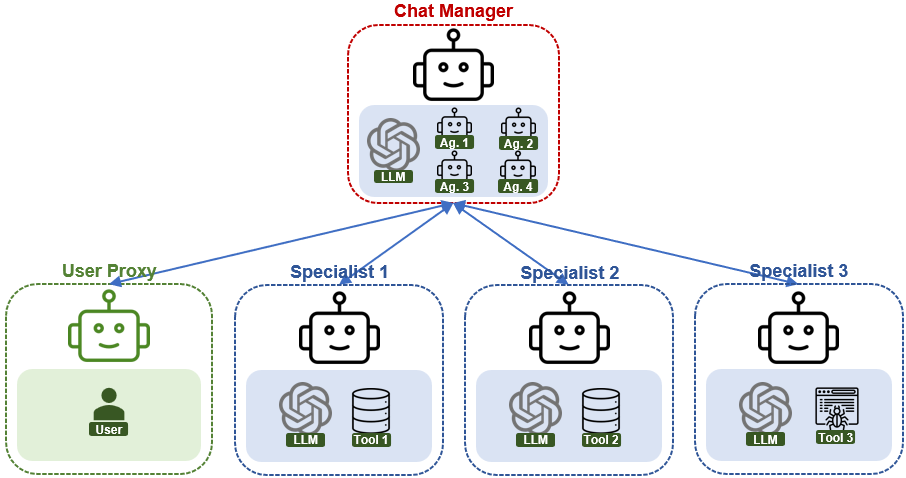
\includegraphics[width=.75\textwidth]{images/agent_config_2.png}
                    \caption{Configuração de chat com um Gerenciador de Chat e um grupo de agentes LLM.}
                    \label{fig:agent_config_2}
                \end{figure}            
                
                \begin{figure}[hbt]
                    \centering
                    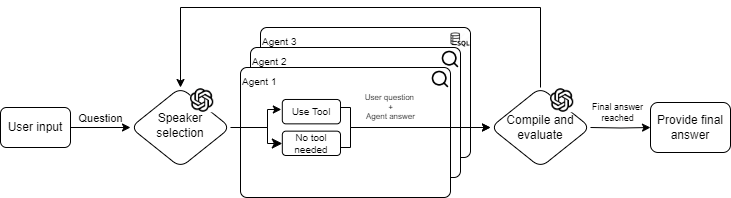
\includegraphics[width=1\textwidth]{images/agent_diagram_2.png}
                    \caption{Processo de decisão multi-agente.}
                    \label{fig:diagrama_agente_MultiAgente_2}
                \end{figure}    
    
                
            \subsection{Avaliação}             
        
                Para o processo de avaliação, em linha com a avaliação conduzida por \cite{Li2023}, um grupo de 3 engenheiros especialistas analisou 33 perguntas e suas respectivas respostas para cada configuração. Os especialistas avaliaram cada par de perguntas e respostas com base nas seguintes métricas predefinidas:
        
                \begin{itemize}
                    
                    \item \textbf{Veracidade:} uma métrica para medir o grau de divergência da precisão factual.
                    
            
                    \item \textbf{Desempenho:} engloba a qualidade geral das respostas, considerando coerência linguística, raciocínio lógico, diversidade e a presença de evidências corroborativas.
                    
                \end{itemize}
                
                A nota final foi determinada pela média das pontuações de todas as entradas para cada configuração. Esta avaliação garantiu uma avaliação abrangente das capacidades dos modelos.
    
    
    \section{Resultados}
    
        Este capítulo fornece uma análise dos dados coletados e responde às perguntas de pesquisa. Os resultados são apresentados na \autoref{tab:tabela_resultados} e estão organizados de acordo com os objetivos do estudo, com cada objetivo sendo abordado em detalhe.
    
        A terceira métrica, Custo do LLM, representa o custo financeiro associado ao uso da API da OpenAI para os modelos de linguagem em cada configuração. Essa métrica é medida em dólares americanos e reflete os recursos computacionais necessários para cada tarefa.            
            
        \begin{table}[h]
            \small % Reduzir o tamanho da fonte
            \centering % Centralizar a tabela na página
            \caption{Resultados nas tarefas de Q\&A e Text-to-SQL, incluindo desvio padrão (Std). As melhores métricas estão destacadas em \textbf{\underline{negrito e sublinhado}}. As segundas melhores estão destacadas em \textbf{negrito}.}
            \label{tab:tabela_resultados}
            \begin{tabular}{|>{\raggedright\arraybackslash}p{2.2cm}|>{\centering\arraybackslash}p{1cm}|>{\centering\arraybackslash}p{1cm}|>{\centering\arraybackslash}p{1cm}|>{\centering\arraybackslash}p{1cm}|>{\centering\arraybackslash}p{1cm}|>{\centering\arraybackslash}p{1cm}|>{\centering\arraybackslash}p{1cm}|>{\centering\arraybackslash}p{1cm}|>{\centering\arraybackslash}p{1cm}|>{\centering\arraybackslash}p{1cm}|}
                \hline
                \rowcolor{gray!20}
                \textbf{Tarefa}           & \multicolumn{5}{c|}{\textbf{Agente Único}}           & \multicolumn{5}{c|}{\textbf{Multi-Agente}} \\ % Mesclando células e adicionando cabeçalho
                \textbf{Modelo}          & \textbf{Custo LLM} & \textbf{Verdade} & \textbf{Std} & \textbf{Desempenho} & \textbf{Std} & \textbf{Custo LLM} & \textbf{Verdade} & \textbf{Std} & \textbf{Desempenho} & \textbf{Std} \\ \hline
                \cellcolor{gray!9} Q\&A & & & & & & & & & &\\
                GPT-3.5-turbo            & 0.005             & 2.94              & 1.48 & 3.94          & 1.09 & 0.02              & 4.09              & 1.22 & 3.82 & 0.98 \\
                GPT-4                   & 0.12              & \textbf{3.88}     & 1.41 & \textbf{4.06} & 1.30 & 0.45              & \underline{\textbf{4.57}} & 0.79 & \underline{\textbf{4.43}} & 0.79 \\
                \cellcolor{gray!9} Text-to-SQL & & & & & & & & & &\\
                GPT-3.5-turbo            & 0.009             & 4.13              & 1.41 & 4.44          & 1.03 & 0.02              & \textbf{4.29}     & 1.20 & \textbf{4.29} & 1.33 \\
                GPT-4                   & 0.10 & \underline{\textbf{4.56}} & 0.96 & \underline{\textbf{4.63}} & 0.81 & 0.51      & 3.20              & 1.99 & 3.70 & 1.89 \\ \hline
            \end{tabular}
        \end{table}
        
        A análise comparativa entre as configurações de agente único e multi-agente para RAG, utilizando os modelos GPT-3.5-turbo e GPT-4, revelou insights sobre as métricas de veracidade, desempenho e custos do modelo de linguagem.
    
    
        
        \subsection{Veracidade} 
        
            Na avaliação da métrica de veracidade, foram observadas diferenças significativas entre os cenários de agente único e multiagente nas tarefas de Perguntas e Respostas (Q\&A) e Text-to-SQL. Os resultados são ilustrados nas Figuras \ref{fig:truthfulness_QA} e \ref{fig:truthfulness_text2sql}. Para as tarefas de Q\&A, o GPT-4 em uma configuração multiagente superou significativamente o desempenho do agente único com uma pontuação de veracidade de 4,57 em comparação com 3,88. O modelo GPT-3.5-turbo apresentou resultados distintos entre as duas configurações, com o multiagente superando o agente único com pontuações de 4,09 e 2,94, respectivamente. 
            
            Em termos de consultas Text-to-SQL, foi observado um resultado diferente. O GPT-4 agente único alcançou uma pontuação de 4,56, enquanto o mesmo modelo na configuração multiagente obteve 3,20, destacando uma limitação do multiagente nessa tarefa. Por outro lado, o GPT-3.5-turbo manteve um desempenho mais equilibrado entre as configurações, pontuando 4,29 para multiagente e 4,13 para agente único.
            
            \begin{figure}[h]
                \centering
                \begin{minipage}{.485\textwidth}
                    \centering           
                    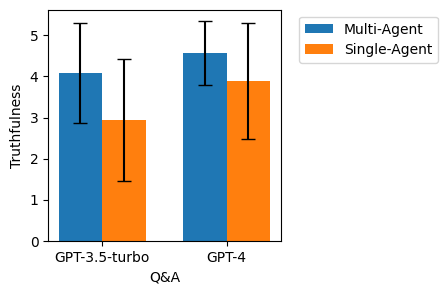
\includegraphics[width=1\linewidth]{images/truthfulness_QA.png}
                    \caption{Veracidade e desvio padrão em tarefas de Q\&A por modelo LLM e configuração de agente. \\ }
                    \label{fig:truthfulness_QA}
                \end{minipage}%
                \hspace{0.2cm}
                \begin{minipage}{.455\textwidth}
                    \centering
                    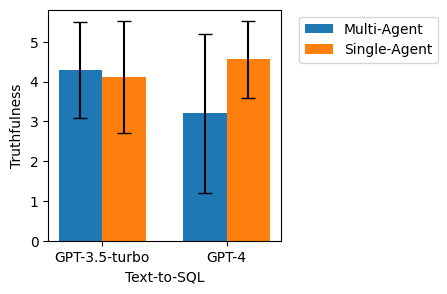
\includegraphics[width=1\linewidth]{images/truthfulness_text2sql.png}
                    \caption{Veracidade e desvio padrão em tarefas de Text-to-SQL por modelo LLM e configuração de agente.}
                    \label{fig:truthfulness_text2sql}
                \end{minipage}
            \end{figure}
    
    
        
        \subsection{Desempenho}
            
            A avaliação do desempenho de LLM \cite{Li2023} nas tarefas de Q\&A e Text-to-SQL revela tendências semelhantes aos resultados de veracidade. Conforme mostrado nas Figuras \ref{fig:performance_QA} e \ref{fig:performance_text2sql} e resumido na Tabela \ref{tab:tabela_resultados}, o desempenho do texto nas configurações de agente único e multiagente foi comparado usando os modelos GPT-3.5-turbo e GPT-4. 
            
            Para as tarefas de Q\&A, a configuração multiagente mostra um aumento de desempenho em comparação com o agente único. Notavelmente, o GPT-4 multiagente alcança uma pontuação de desempenho de 4,43, que é superior à pontuação de 4,06 do GPT-4 agente único. Esse padrão é consistente com o GPT-3.5-turbo, onde o sistema multiagente também supera o sistema de agente único, pontuando 3,82 e 3,94, respectivamente. Esses achados enfatizam a eficácia da abordagem multiagente em lidar com consultas técnicas dos usuários.
            
            \begin{figure}[h]
                \centering
                \begin{minipage}{.48\textwidth}
                    \centering                
                    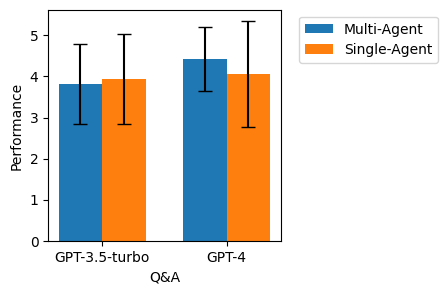
\includegraphics[width=1\linewidth]{images/performance_QA.png}
                    \caption{Desempenho e desvio padrão em tarefas de Q\&A por modelo LLM e configuração de agente.\\}
                    \label{fig:performance_QA}
                \end{minipage}
                \hspace{0.2cm}
                \begin{minipage}{.48\textwidth}
                    \centering
                    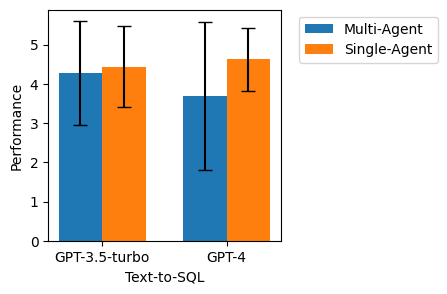
\includegraphics[width=1\linewidth]{images/performance_text2sql.png}
                    \caption{Desempenho e desvio padrão em tarefas de Text-to-SQL por modelo LLM e configuração de agente.}
                    \label{fig:performance_text2sql}
                \end{minipage}%
            \end{figure}
            
        \subsection{Custo de LLM}
        
            Os serviços de modelos de linguagem são tipicamente compostos por valores por token. Por exemplo, o modelo GPT-4 custa US\$30,00 (entrada) e US\$60,00 (saída) por 1 milhão de tokens recebidos e enviados, respectivamente.
            
            A arquitetura de agente único demonstrou custos substancialmente mais baixos para as tarefas de Q\&A e Text-to-SQL em comparação com a configuração multiagente, conforme mostrado na Figura~\ref{fig:truthfulness_vs_cost_vs_config_model}. Por exemplo, o custo médio do modelo GPT-4 \cite{OpenAI2023} para uma tarefa de Q\&A foi de \$0,12 por pergunta processada para o agente único, enquanto o multiagente registrou um custo médio de \$0,45. Essa tendência de custos mais altos para a arquitetura multiagente também foi mantida para tarefas de Text-to-SQL, com um custo médio de \$0,51 para a arquitetura multiagente em contraste com \$0,10 para o agente único.
            
            O maior número de tokens e custo para a configuração multiagente deve-se à inclusão de chamadas intermediárias, por exemplo, quando o "Selector de Agentes" precisa decidir para qual agente passar a vez. Todo o histórico de mensagens é passado para o LLM nesse estágio, aumentando substancialmente o número de tokens submetidos e o tempo de resposta.
            
            \begin{figure}[h]
                \centering              
                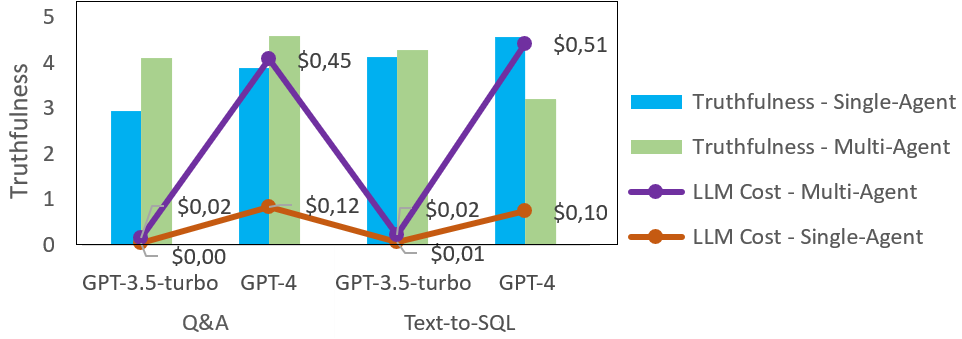
\includegraphics[width=0.75\textwidth]{images/truthfulness_vs_cost_vs_config_model.png}
                \caption{Custos médios de LLM e Veracidade por tarefa concluída de acordo com a configuração e modelo.}
                \label{fig:truthfulness_vs_cost_vs_config_model}
            \end{figure}
    
    
    \section{Discussão} 
        
        A comparação entre sistemas de agente único e multiagente revelou diferenças significativas em termos de desempenho e custo:
        
        \subsection{Desempenho Geral.}     
            Os resultados indicam que, para tarefas de Q\&A no contexto de O\&G, a medida de veracidade foi 28\% maior com a arquitetura multiagente em comparação com a de agente único. No entanto, para tarefas de Text-to-SQL, essa tendência foi invertida, onde o agente único obteve uma pontuação 15\% maior.
            
            Esses achados sugerem que, para tarefas de Q\&A, a configuração multiagente pode ser mais vantajosa em termos de fornecer informações verídicas, especialmente ao utilizar o modelo mais avançado GPT-4. Em contrapartida, nas tarefas de Text-to-SQL, o modelo GPT-4 em uma configuração de agente único provou ser mais eficaz. Isso pode implicar que a complexidade adicional de gerenciar múltiplos agentes em algumas tarefas não leva necessariamente a um desempenho melhor nas respostas, ressaltando a importância de selecionar cuidadosamente a configuração do agente com base no tipo de tarefa e nas características específicas do modelo de linguagem utilizado.
            
        \subsection{Análise de Custo-Desempenho.}
        
            Embora o sistema multiagente mostre maior veracidade nas tarefas de Q\&A, é crucial considerar os custos associados. Para fornecer uma comparação mais clara, considere as razões pontuação/custo. Para tarefas de Q\&A usando GPT-4, a configuração de agente único produz uma razão de 32,33 pontos de veracidade por dólar, comparado a 10,16 para a configuração multiagente. Isso indica que, embora o sistema multiagente mostre uma melhoria de 17,8\% na veracidade, isso ocorre com um aumento de custo de 275\%.
            
            Com base em nossa análise, recomendamos o uso de um sistema multiagente para tarefas de Q\&A quando o orçamento permitir e a precisão for um fator crítico. No entanto, os tomadores de decisão devem considerar a definição de um limite de custo-desempenho para orientar a escolha da configuração do sistema, garantindo que os benefícios justifiquem os gastos envolvidos.
        
        \subsection{Variações no Desempenho dos Modelos.}
            Curiosamente, nossos resultados mostram que o GPT-3.5-turbo supera o GPT-4 em certas tarefas, particularmente na configuração multiagente de Text-to-SQL, apesar do maior tamanho e treinamento mais extenso do GPT-4. Esse desempenho inesperado pode ser atribuído a vários fatores. Primeiro, o GPT-3.5-turbo pode ter passado por um ajuste fino mais específico para tarefas de consulta estruturada, permitindo que ele se destaque em cenários de Text-to-SQL. Além disso, os dados de treinamento do GPT-3.5-turbo podem ser mais recentes ou mais relevantes para o domínio específico do nosso estudo. Outra possibilidade é que o menor tamanho do modelo GPT-3.5-turbo permita um processamento mais rápido e um manuseio mais eficiente da configuração multiagente, resultando em melhor desempenho em alguns contextos.
            
            No entanto, é importante notar que o GPT-4, quando usado em uma configuração multiagente, demonstrou uma veracidade e um desempenho mais consistentes, como evidenciado por sua redução no desvio padrão nos resultados. Essa consistência pode ser particularmente vantajosa em aplicações onde confiabilidade e precisão são críticas. Sistemas multiagentes têm a vantagem de manter contextos separados para diferentes aspectos de uma tarefa. Essa compartimentalização pode levar a um melhor manuseio de consultas complexas e multifacetadas, à medida que cada agente pode se concentrar em seu contexto específico sem ser sobrecarregado por informações irrelevantes. No entanto, essa vantagem pode ser compensada em tarefas como Text-to-SQL, onde manter um contexto unificado do esquema do banco de dados e da estrutura da consulta é crucial, possivelmente explicando o melhor desempenho das configurações de agente único nessa tarefa.
            
            A arquitetura multiagente envolve inerentemente múltiplos estágios de processamento de informações, que podem servir como mecanismos naturais de filtragem. À medida que a informação passa de um agente para outro, dados irrelevantes ou de baixa qualidade podem ser naturalmente filtrados, levando a saídas finais mais refinadas e precisas. Isso pode explicar o desempenho superior na filtragem de informações irrelevantes observado nas configurações multiagentes.
    
    
    
        \subsection{Eficiência Econômica.}
        
            A arquitetura multiagente incorre em custos significativamente mais altos em comparação com o sistema de agente único, principalmente devido a chamadas intermediárias adicionais ao modelo de linguagem e múltiplas iterações entre agentes para o planejamento de ações. As diferenças de custo entre o uso do GPT-4 e do GPT-3.5-turbo são substanciais, com o GPT-4 sendo notavelmente mais caro.
            
            Conforme detalhado na seção Análise de Custo-Desempenho, a razão de veracidade por dólar destaca os trade-offs econômicos entre sistemas de agente único e multiagente. Embora o sistema multiagente ofereça melhorias na veracidade, isso vem com um aumento considerável de custo, impactando a eficiência econômica geral.
            
            Para uma grande empresa com 40.000 trabalhadores do conhecimento, a escolha do modelo e da arquitetura impacta significativamente os custos anuais. Usar o GPT-4 em uma configuração de agente único poderia resultar em um custo anual de aproximadamente \$4,38 milhões, enquanto o GPT-3.5 custaria cerca de \$438.000. No entanto, ao empregar uma arquitetura multiagente, os custos aumentam substancialmente. A configuração multiagente com GPT-4 elevaria o custo anual para \$16,425 milhões, representando um aumento dramático devido ao uso de tokens 3,75 vezes maior. Da mesma forma, o GPT-3.5 em uma configuração multiagente custaria \$1,642 milhões. Essas estimativas assumem um padrão médio de uso de 10.000 tokens por trabalhador por dia e ressaltam as implicações financeiras significativas da adoção de um sistema multiagente, que, embora possa oferecer benefícios de desempenho, vem com um aumento considerável nos custos de LLM.
            
            Em resumo, enquanto sistemas multiagentes e modelos mais avançados como o GPT-4 oferecem melhorias no desempenho, a eficiência econômica, medida pela veracidade por dólar, pode favorecer sistemas de agente único e modelos menos custosos como o GPT-3.5-turbo, dependendo da aplicação específica e das restrições orçamentárias.
            
        \subsection{Desafios e Limitações.}  
        
            Durante a avaliação dos agentes, vários desafios e limitações foram identificados.
            
            \begin{itemize}
                \item \textbf{Contextualização e Interpretação}: 
                    Em muitos casos, a solução de agente único teve dificuldades para entender o contexto da pergunta. Por exemplo, uma pergunta sobre cimentação foi interpretada no contexto da indústria da construção, um tema ao qual os modelos de linguagem foram mais expostos durante a fase de treinamento. No entanto, a estrutura multiagente, com seus papéis bem definidos, compreendeu melhor as perguntas e mostrou desempenho superior nas tarefas de Q\&A, corroborando os achados de \cite{Li2024}.
    
                
                \item \textbf{Filtragem de Informações Irrelevantes}: 
                
                    O agente frequentemente recebe documentos irrelevantes junto com os importantes no contexto do prompt, e cabe ao LLM ignorá-los. Por exemplo, quando perguntado sobre alternativas para acelerar o tempo de cura da pasta de cimento sem comprometer sua integridade em altas temperaturas, o sistema RAG recuperou um documento que incluía informações sobre cimentação em lote para garantir homogeneidade durante a fabricação e bombeamento. Embora essa informação seja verdadeira, não era relevante para a pergunta específica feita. Nesse aspecto, a solução multiagente teve um desempenho melhor ao descartar tais informações irrelevantes, focando mais precisamente na tarefa em questão. Outras possíveis soluções incluem melhorar a precisão da busca semântica ajustando um limite mínimo para medidas de similaridade ou por meio de técnicas de reclassificação, como as propostas por \cite{Carraro2024} e \cite{Sun2023}.
                
            
                \item \textbf{Alucinação}: 
                
                    Durante a avaliação do nosso sistema, encontramos instâncias em que o agente produziu informações alucinadas em vez de utilizar a ferramenta apropriada para recuperar dados precisos, como em \cite{Bilbao2023}. Por exemplo, quando perguntado "Quantas anomalias ocorreram na sonda número 05 durante agosto de 2023?", esperava-se que o agente usasse a ferramenta Text-to-SQL para consultar o banco de dados. No entanto, ele ignorou essa ferramenta e gerou uma resposta fabricada, afirmando que ocorreram 5 anomalias, juntamente com descrições detalhadas de eventos fictícios. A resposta correta, conforme recuperada do banco de dados, foi que ocorreram 7 anomalias. Essa alucinação provavelmente resultou da dependência do agente em seu conhecimento interno em vez da recuperação de dados externos.
                    \item Em termos de estatísticas de alucinação, nossa análise revelou que para tarefas de Q\&A, as alucinações ocorreram em 9,6\% dos casos e 3,8\% foram parcialmente alucinadas. Em contraste, as tarefas de Text-to-SQL exibiram uma taxa de alucinação menor, com apenas 3,6\% das respostas contendo informações alucinadas e 96,4\% sendo precisas. Esses achados destacam a suscetibilidade variável à alucinação entre diferentes tipos de tarefas, enfatizando a necessidade de estratégias direcionadas para mitigar esse problema.
                
            
                \item \textbf{Jargão da Indústria}:
                
                    Analisando especificamente a atividade de perfuração e completação de poços offshore, o principal desafio é a natureza inerentemente complexa e técnica dos dados envolvidos. 
                    Houve instâncias de interpretação incorreta da informação, provavelmente devido ao uso de termos, expressões e temas específicos da construção de poços, aos quais o modelo de linguagem teve pouca ou nenhuma exposição durante a fase de treinamento. 
                    Uma possível solução é a implementação de modelos especializados, que tem sido apontada na literatura cinza como uma tendência para os próximos anos \cite{Shah2024, Meena2023, Ghosh2023}.
                
            
                \item \textbf{Ferramentas vs. Desempenho}: 
                
                    Foi identificado durante os experimentos que agentes com uma alta quantidade de ferramentas mostraram um declínio no desempenho geral. Isso pode ser atribuído ao contexto adicionado aos prompts. À medida que o comprimento do contexto aumenta, a capacidade do modelo de interpretar e responder com precisão diminui. Esta é uma limitação dos modelos de linguagem atuais, onde contextos mais longos podem levar a uma diluição de informações relevantes e aumentar a dificuldade em manter a coerência e a precisão. Esta conclusão é atualmente qualitativa, pois essas métricas não foram abordadas neste experimento.
                
            
                \item \textbf{Consultas Envolvendo Nomes Próprios}:
                
                    Em consultas envolvendo nomes de pessoas, não foi possível recuperar documentos relevantes usando a busca semântica. Por exemplo, quando solicitado a identificar o funcionário associado a uma chave específica e listar os itens de conhecimento que registraram no sistema, o sistema RAG atribuiu incorretamente itens de conhecimento ao autor errado. Isso destaca a dificuldade em recuperar informações com precisão baseadas em nomes próprios, que podem ser complicadas por variações em acentuação, abreviação e formatação.
                    Uma solução potencial a ser explorada é o uso do Self-Query Retriever \cite{LangchainSelfQuery2023}, implementando uma busca híbrida com filtros de metadados (incluindo nomes próprios) e recuperação semântica do restante da consulta. Também é sugerido, nesses casos, usar a distância de \cite{Levenshtein1966} para lidar com possíveis variações na grafia dos nomes. Essa abordagem poderia melhorar a precisão na recuperação de documentos relacionados a indivíduos específicos, garantindo que as informações corretas sejam associadas à pessoa certa.
                
            \end{itemize}
            
    
        \subsection{Implicações Práticas.} 
            Os achados do nosso estudo têm implicações práticas significativas para o setor de O\&G e, potencialmente, para outras indústrias caracterizadas por ambientes de dados complexos e técnicos:
            
            \begin{itemize}
                \item \textbf{Apoio Aprimorado à Tomada de Decisões:}            
                    Nossos resultados indicam que sistemas multiagentes fornecem uma medida de veracidade 28\% maior em tarefas de Q\&A. Isso pode ser particularmente benéfico para a tomada de decisões em engenharia de poços, onde informações precisas e verídicas são críticas.
                    Implementar sistemas multiagentes nos processos de tomada de decisão pode levar a decisões mais confiáveis e informadas, reduzindo o risco de erros e aumentando a segurança e eficiência operacional.
                
                
                \item \textbf{Equilíbrio entre Desempenho e Eficiência Econômica:}          
                    Embora sistemas multiagentes ofereçam desempenho superior em termos de veracidade, eles vêm com um custo que é, em média, 3,7 vezes maior em comparação com sistemas de agente único.
                    Isso destaca a importância de uma abordagem estratégica na seleção de configurações de agentes com base em tarefas específicas e restrições orçamentárias.
                    Uma análise detalhada de custo-benefício revela que, para tarefas de Q\&A usando GPT-4, a configuração de agente único produz uma razão de 32,33 pontos de veracidade por dólar, comparado a 10,16 para a configuração multiagente. Enquanto o sistema multiagente mostra uma melhoria de 17,8\% na veracidade, isso vem com um aumento de custo de 275\%. A eficiência varia significativamente por tipo de tarefa; em tarefas de Text-to-SQL, o GPT-4 agente único supera o multiagente em 42,5\% na veracidade enquanto custa 80,4\% menos.
                
            
                \item \textbf{Agentes de Reflexão e Crítica:}            
                    Uma abordagem promissora para melhorar o desempenho desses agentes é o uso da reflexão \cite{Shinn2023}, um método onde os agentes refletem verbalmente sobre sinais de feedback da tarefa e mantêm esse texto reflexivo em um buffer de memória episódica para melhorar a tomada de decisões em tentativas subsequentes.
                    Agentes críticos são uma forma de implementar a reflexão em uma configuração multiagente. Esse tipo de agente é desafiador de aplicar em tarefas de Q\&A sobre dados técnicos privados, pois LLMs comerciais (OpenAI, Google Bard e outros) não foram profundamente treinados no domínio e têm dificuldade em fornecer críticas relevantes e precisas, reforçando a tendência de uso crescente de modelos específicos de domínio \cite{Shah2024, Meena2023, Ghosh2023}.
                
            
                \item \textbf{Configuração de Agentes Específica para a Tarefa:}            
                    O estudo destaca que a complexidade de gerenciar múltiplos agentes nem sempre leva a um desempenho melhor. Em alguns casos, uma configuração de agente único pode ser mais eficaz.
                    Essa percepção pode orientar o desenvolvimento e a implantação de sistemas de IA, garantindo que a configuração dos agentes seja adaptada aos requisitos específicos da tarefa, otimizando tanto o desempenho quanto o custo.
                
            
                \item \textbf{Potencial para Aplicação Ampla:}            
                    As percepções obtidas deste estudo não se limitam ao setor de O\&G, mas podem ser aplicadas a outras indústrias com complexidades técnicas similares, como aeroespacial, farmacêutica e energia renovável.
                    Ao adotar sistemas multiagentes nessas indústrias, as organizações podem melhorar a tomada de decisões, a gestão do conhecimento e a eficiência operacional, impulsionando a inovação e a competitividade.
                             
            \end{itemize}
    
    
        \subsection{Futuras Direções}
        
            Este trabalho indica possíveis caminhos para aprimorar as arquiteturas RAG no setor de O\&G.
            
            \begin{itemize}
            
                \item \textbf{Aprimoramento das Técnicas Semânticas de IR:}
                    Há uma necessidade crítica de desenvolver tecnologias de busca semântica mais sofisticadas. Esforços futuros devem se concentrar em aumentar a precisão da recuperação de informações, filtrando conteúdos irrelevantes de maneira mais eficaz. Isso garantirá que os agentes possam fornecer respostas mais precisas e contextualmente adequadas, crucial para domínios técnicos como O\&G.
                    
                \item \textbf{Desenvolvimento de Modelos Específicos de Domínio:}
                     Modelos especializados, feitos especificamente para O\&G e outros domínios, como engenharia biomédica \cite{Pal2024}, poderiam melhorar significativamente o manuseio de jargões específicos e dados técnicos complexos, ao mesmo tempo que reduzem os custos de LLM \cite{Arefeen2024}. Pesquisas futuras devem visar desenvolver e treinar esses modelos para entender e interpretar melhor a linguagem e os tipos de dados únicos encontrados em O\&G, melhorando a precisão geral das respostas dos agentes.
                    
                \item \textbf{Otimização do Uso de Ferramentas no Desempenho dos Agentes:}
                    A relação entre a quantidade de ferramentas disponíveis para um agente e seu desempenho precisa de mais exploração. Estudos futuros devem quantificar o impacto da disponibilidade de ferramentas na eficácia e eficiência do agente, visando otimizar o uso das ferramentas sem sobrecarregar o agente ou diluir a qualidade do desempenho.
                    
                \item \textbf{Integração de Técnicas Avançadas de Reconhecimento de Nomes:}
                    Consultas que envolvem nomes próprios representam um desafio significativo na busca semântica. A integração de técnicas avançadas de recuperação, como Self-Query Retrievers \cite{LangchainSelfQuery2023} e algoritmos de distância \cite{Levenshtein1966}, poderia melhorar o tratamento dessas consultas. Pesquisas futuras devem se concentrar em aprimorar as capacidades de reconhecimento de nomes para garantir que os agentes possam recuperar e utilizar informações corretas com precisão, especialmente em cenários onde a precisão é fundamental.
                    
                \item \textbf{Extensão para Outros Domínios Complexos:}
                    As potenciais aplicações de sistemas multiagentes não se limitam ao setor de O\&G. Pesquisas futuras devem explorar a adaptação e implementação desses sistemas em outros domínios complexos e técnicos, como aeroespacial, farmacêutico e energia renovável. Investigar como esses sistemas podem apoiar a tomada de decisões nessas áreas fornecerá insights valiosos sobre sua versatilidade e adaptabilidade.
                    
                \item \textbf{Experimentação com Modelos Híbridos:}
                    Combinar as forças de sistemas de agente único e multiagente pode trazer benefícios significativos. As direções futuras devem incluir a experimentação com modelos híbridos que integrem a robustez e profundidade das interações multiagentes com a simplicidade e eficiência dos sistemas de agente único. Essa abordagem híbrida poderia potencialmente oferecer uma solução equilibrada, maximizando o desempenho enquanto gerencia custos e complexidade.
            
            \end{itemize}
            
            Ao seguir essas direções, a pesquisa futura pode avançar significativamente no desenvolvimento de sistemas multiagentes, não apenas aprimorando sua aplicação no setor de O\&G, mas também expandindo sua utilidade em várias atividades tecnologicamente intensivas.
    
    


\chapter{Experimento 2}
    

    \section{Metodologia 2}
        
        ...

        \begin{algorithm}
            \caption{Experiment Execution Loop}
            \begin{algorithmic}[1]
            \Require questions, setups, models
            \Ensure results
            
            \Function{RunExperiment}{}
                \State $results \gets \{\}$
                
                \ForAll{$question \in questions$}
                    \State $ground\_truth \gets question.ground\_truth$
                    
                    \ForAll{$setup \in setups$}
                        \ForAll{$model \in models$}
                            \State $agent \gets \text{InitializeAgent}(setup, model)$
                            \State $response \gets agent.\text{ProcessQuestion}(question)$
                            
                            \State $metrics \gets \text{EvaluateResponse}(response, ground\_truth)$
                            
                            \State $results[question, setup, model] \gets \{$
                            \State \hspace{1cm} $"response": response,$
                            \State \hspace{1cm} $"metrics": metrics,$
                            \State \hspace{1cm} $"execution\_trace": agent.trace$
                            \State $\}$
                        \EndFor
                    \EndFor
                \EndFor
                
                \State \Return $\text{AggregateResults}(results)$
            \EndFunction
            
            % \Function{ProcessQuestion}{$question$}
            %     \State $state \gets \text{Initialize}(question)$
                
            %     \While{$\text{not IsComplete}()$}
            %         \State $action \gets \text{DetermineNextAction}(state)$
                    
            %         \If{$\text{IsToolCall}(action)$}
            %             \State $result \gets \text{ExecuteTool}(action.tool, action.parameters)$
            %             \State $state \gets \text{UpdateState}(state, result)$
            %         \Else
            %             \State $state \gets \text{UpdateReasoning}(state)$
            %         \EndIf
            %     \EndWhile
                
            %     \State \Return $\text{GenerateFinalAnswer}(state)$
            % \EndFunction
            
            % \Function{EvaluateResponse}{$response, ground\_truth$}
            %     \State \Return $\{$
            %     \State \hspace{0.5cm} $"accuracy": \text{CalculateAccuracy}(response, ground\_truth),$
            %     \State \hspace{0.5cm} $"precision": \text{CalculatePrecision}(response, ground\_truth),$
            %     \State \hspace{0.5cm} $"recall": \text{CalculateRecall}(response, ground\_truth),$
            %     \State \hspace{0.5cm} $"f1\_score": \text{CalculateF1}(response, ground\_truth),$
            %     \State \hspace{0.5cm} $"answer\_size\_ratio": \text{CalculateSizeRatio}(response, ground\_truth)$
            %     \State $\}$
            % \EndFunction
            \end{algorithmic}
        \end{algorithm}
            
        \subsection{Dataset de Q\&A}

            ...
        
        \subsection{Setups}
        
            \subsubsection{Linear-Flow with Router}        
                ...
            
            \subsubsection{Single-Agent}        
                ...
            
            \subsubsection{Multi-Agent}        
                ...
            
        \subsection{Frameworks utilizados}
        
            ...
            
        \subsection{Avaliação de desempenho}

            [Falar brevemente sobre métricas, prompts, citar ragas, etc]
            


    \section{Resultados 2}
        
        \subsubsection{Geral}

            [GERAR TEXTO AQUI]

            ...

            ...
            
            ...

            [GERAR GRÁFICO NOVO AQUI onde config são as cores e X os modelos]
            
            \begin{figure}[h!]
                \centering              
                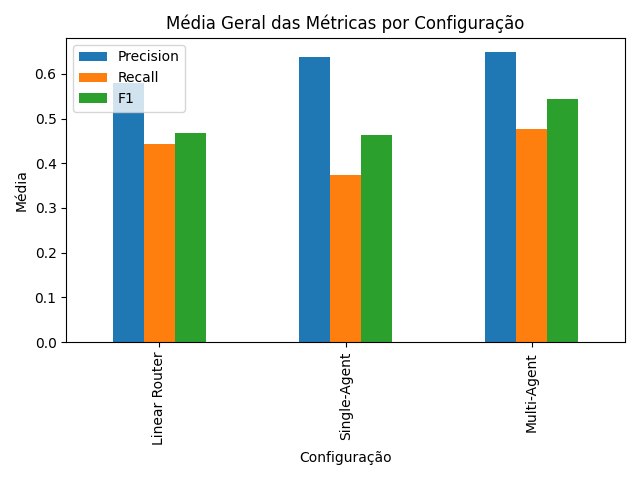
\includegraphics[width=0.75\textwidth]{images_part_2/media_geral_por_configuracao.png}
                \caption{Precisão, recall e f1 por configuração.             [GERAR GRÁFICO NOVO AQUI]}
                \label{fig:aaaa}
            \end{figure}


            ...
            
            ...

            ...
        
        \subsubsection{F1 Score}
        
            
            [GERAR TEXTO AQUI]

            ...

            ...

            ...
            
            % \begin{figure}
            %     \centering
            %     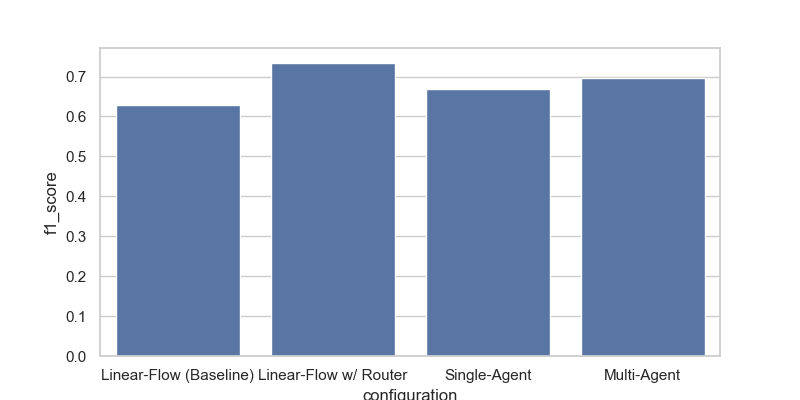
\includegraphics[width=0.5\linewidth]{images_exp2/bar_avg_f1_by_configuration.png}
            %     \caption{Average F1 by RAG architecture.}
            %     \label{fig:enter-label}
            % \end{figure}

            % \begin{figure}
            %     \centering
            %     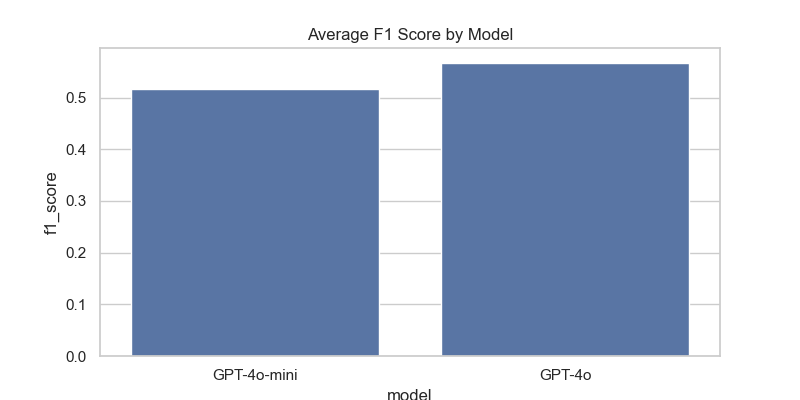
\includegraphics[width=0.5\linewidth]{images_exp2/bar_avg_f1_by_model.png}
            %     \caption{Average F1 Score by language model.}
            %     \label{fig:enter-label}
            % \end{figure}            
            \begin{figure}[h]
              \centering
              \begin{minipage}{0.45\textwidth}
                \centering
                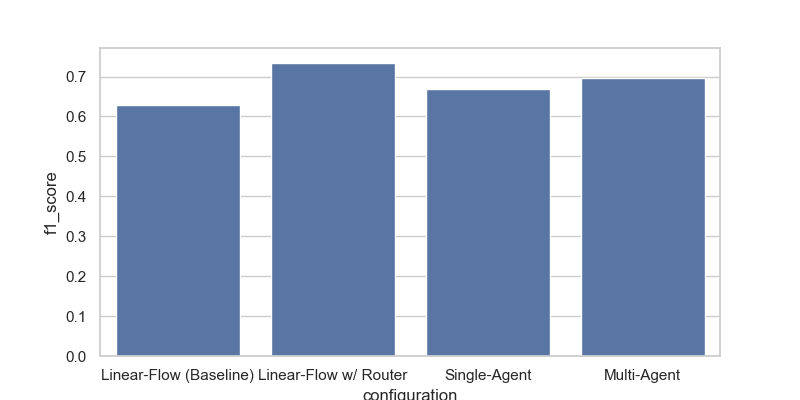
\includegraphics[width=\textwidth]{images_exp2/bar_avg_f1_by_configuration.png}
                \caption{Image 1 caption}
                \label{fig:image1}
              \end{minipage}
              \hfill
              \begin{minipage}{0.45\textwidth}
                \centering
                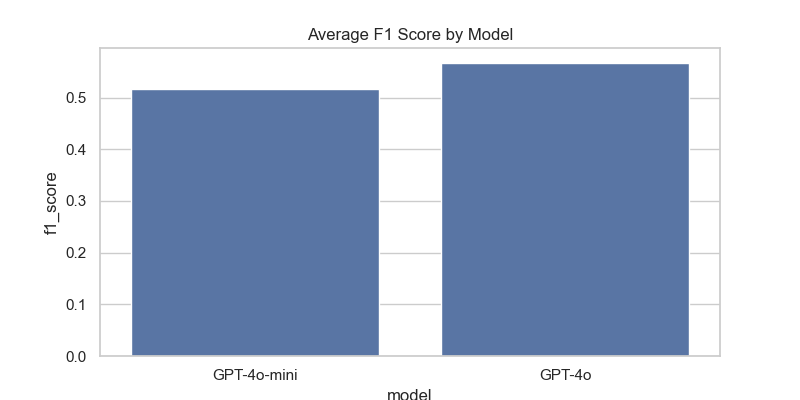
\includegraphics[width=\textwidth]{images_exp2/bar_avg_f1_by_model.png}
                \caption{Image 2 caption}
                \label{fig:image2}
              \end{minipage}
            \end{figure}
            
            
            [GERAR TEXTO AQUI]

            ...

            ...

            ...
            % \begin{figure}[h!]
            %     \centering              
            %     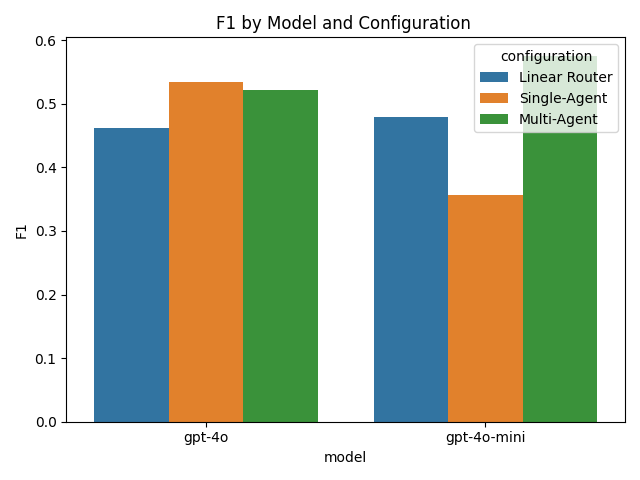
\includegraphics[width=0.75\textwidth]{images_part_2/model_f1_model_configuration.png}
            %     \caption{F1 Score por modelo e configuração.}
            %     \label{fig:aaaa}
            % \end{figure}
            \begin{figure}
                % \centering
                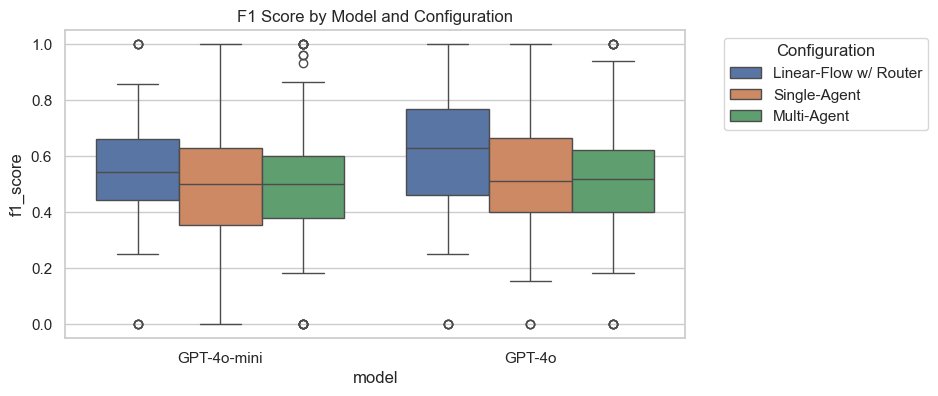
\includegraphics[width=1.1\linewidth]{images_exp2/f1_score_by_model_and_configuration.png}
                \caption{F1 Score distribution by model and configuration of agents}
                \label{fig:f1_score_by_model_and_configuration}
            \end{figure}
                
            [GERAR TEXTO AQUI]

            ...

            ...

            ...
            
            
            \begin{figure}
                \centering
                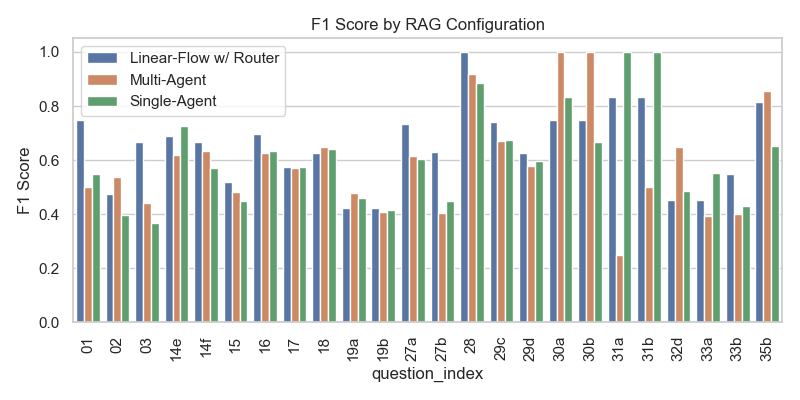
\includegraphics[width=1\linewidth]{images_exp2/best_f1_by_question_index_and_configuration.png}
                \caption{Enter Caption}
                \label{fig:enter-label}
            \end{figure}
            
            [GERAR TEXTO AQUI]

            ...

            ...

            ...
            
            % \begin{figure}[h!]
            %     \centering              
            %     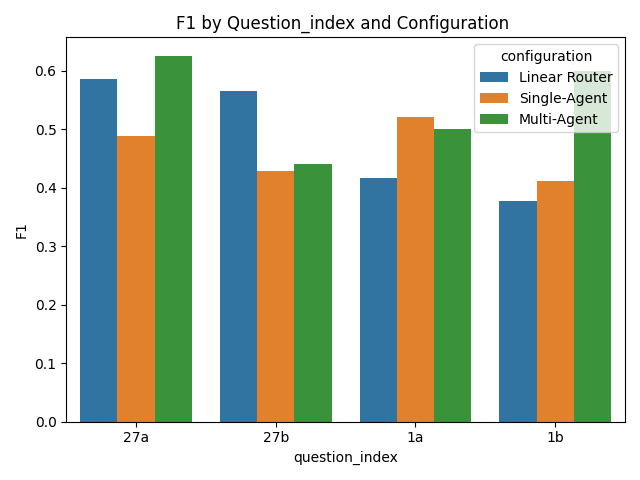
\includegraphics[width=0.75\textwidth]{images_part_2/question_f1_question_index_configuration.png}
            %     \caption{F1 Score por pergunta e configuração.}
            %     \label{fig:aaaa}
            % \end{figure}


            [GERAR TEXTO AQUI]

            ...

            ...
            
            ...

            
            \begin{figure}
                \centering
                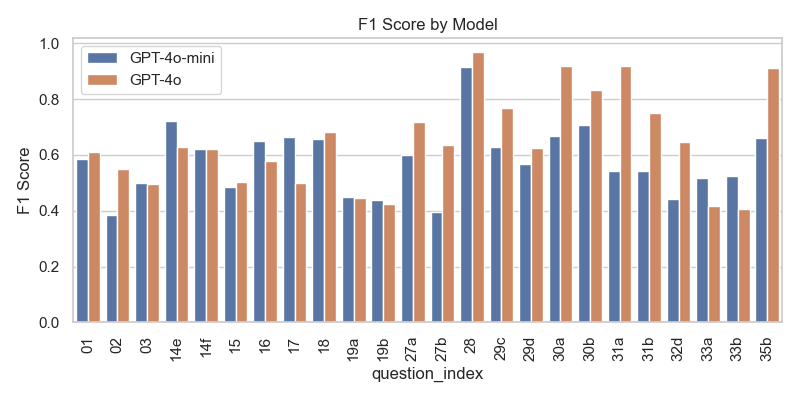
\includegraphics[width=1\linewidth]{images_exp2/best_f1_by_question_index_and_model.png}
                \caption{Enter Caption}
                \label{fig:enter-label}
            \end{figure}


        \subsubsection{Precisão}

            [GERAR TEXTO AQUI]

            ...

            ...

            ...

            \begin{figure}[h!]
                \centering              
                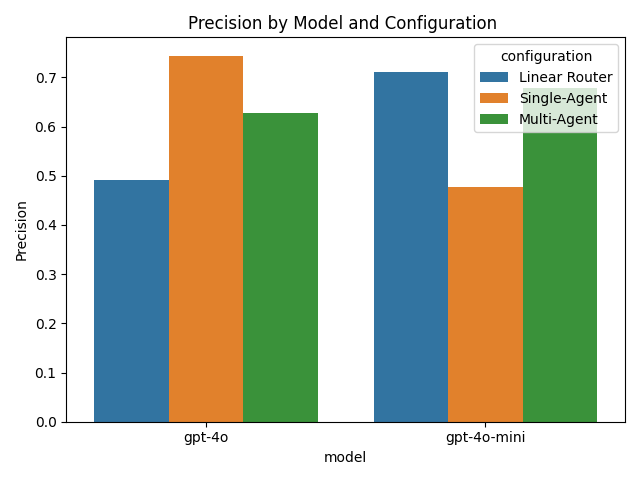
\includegraphics[width=0.75\textwidth]{images_part_2/model_precision_model_configuration.png}
                \caption{Precisão por modelo e configuração.}
                \label{fig:aaaa}
            \end{figure}
            
            [GERAR TEXTO AQUI]

            ...

            ...

            ...

            \begin{figure}[h!]
                \centering              
                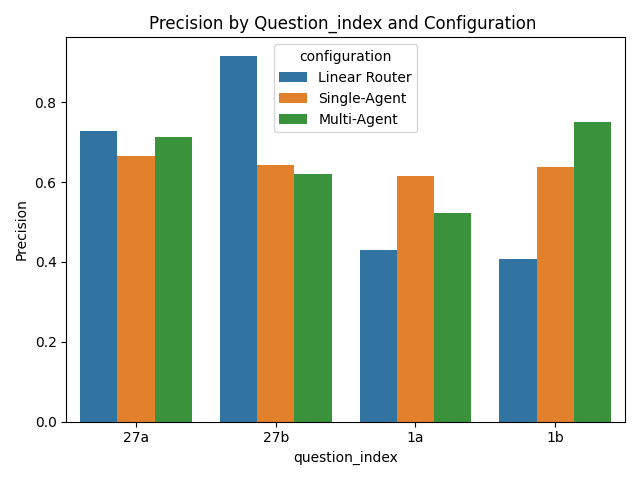
\includegraphics[width=0.75\textwidth]{images_part_2/question_precision_question_index_configuration.png}
                \caption{Precisão por pergunta e configuração.}
                \label{fig:aaaa}
            \end{figure}    

            [GERAR TEXTO AQUI]

            ...

            ...

        
        \subsubsection{Recall}
        
            [GERAR TEXTO AQUI]

            ...

            ...
            
            \begin{figure}[h!]
                \centering              
                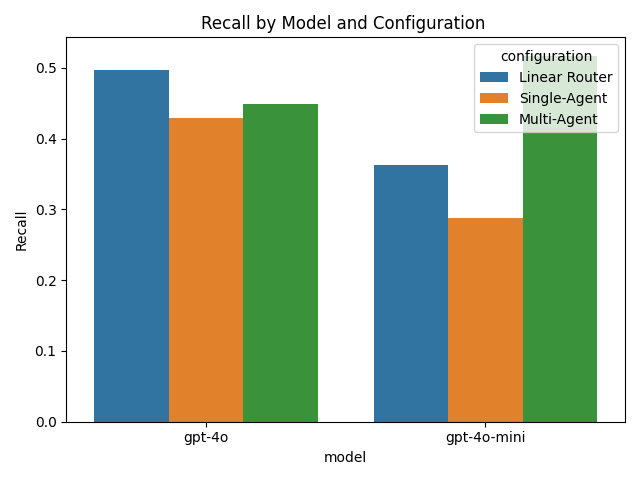
\includegraphics[width=0.75\textwidth]{images_part_2/model_recall_model_configuration.png}
                \caption{Recall por modelo e configuração.}
                \label{fig:aaaa}
            \end{figure}

            [GERAR TEXTO AQUI]

            ...

            ...

            ...
            
            \begin{figure}[h!]
                \centering              
                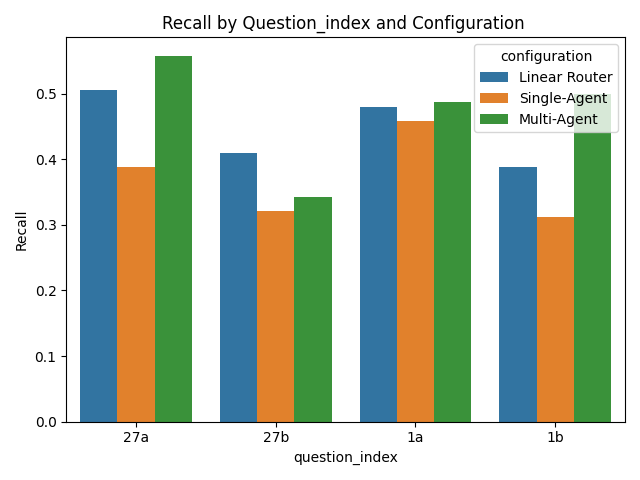
\includegraphics[width=0.75\textwidth]{images_part_2/question_recall_question_index_configuration.png}
                \caption{Recall por pergunta e configuração.}
                \label{fig:aaaa}
            \end{figure}

            [GERAR TEXTO AQUI]

            ...

            ...
        
    \section{Discussão 2}
        
            [GERAR TEXTO AQUI]

            ...
            
            ...
        
        \subsection{aaaa}

            [GERAR TEXTO AQUI]

            ...
            
            ...
        
        \subsection{aaaa}
        
            [GERAR TEXTO AQUI]

            ...
            
            ...
            
        \subsection{aaaa}
        
            [GERAR TEXTO AQUI]

            ...
            
            ...
            
        \subsection{aaaa}
        
            [GERAR TEXTO AQUI]

            ...
            
            ...


\chapter{Conclusões}

    Os resultados deste estudo destacam o potencial das arquiteturas multiagente baseadas em LLMs no setor de O\&G, especialmente no domínio da engenharia de poços. A capacidade de processar e responder a consultas complexas abre caminho para uma transformação digital significativa na área.
    
    Nossa análise comparativa de arquiteturas de agente único e multiagente, utilizando GPT-3.5-turbo e GPT-4, revela um panorama detalhado de trade-offs entre desempenho e eficiência econômica. Os sistemas multiagente demonstram uma veracidade 28\% maior em tarefas de perguntas e respostas (Q\&A), especialmente com GPT-4, em comparação com sistemas de agente único. No entanto, eles incorrem em custos de LLM que são, em média, 3,7 vezes maiores devido às complexidades da comunicação entre agentes. Em contraste, os sistemas de agente único se destacam em tarefas de Text-to-SQL, apresentando um desempenho 15\% melhor do que as configurações multiagente. Essa dinâmica de custo-benefício exige uma consideração cuidadosa ao implementar RAG em cenários do mundo real, onde precisão e restrições financeiras devem ser equilibradas.
    
    Destacamos vários desafios encontrados durante nossos experimentos, incluindo questões de contextualização, necessidade de filtragem de informações mais refinada e a persistência de alucinações. Esses desafios sublinham a necessidade de pesquisas contínuas em áreas como modelos especializados em domínios específicos, técnicas avançadas de busca semântica e arquiteturas híbridas que combinem as forças dos sistemas de agente único e multiagente.
    
    As implicações práticas deste estudo vão além do setor de O\&G. Os insights alcançados aqui são aplicáveis a qualquer domínio intensivo em conhecimento que lide com grandes volumes de dados técnicos. Ao focar em aprimorar os mecanismos de recuperação, desenvolver LLMs específicos de domínio e otimizar as interações entre agentes e ferramentas, pavimentamos o caminho para soluções RAG mais eficazes, confiáveis e econômicas em diversos setores.
    
    Os principais pontos do estudo são os seguintes: sistemas multiagente oferecem superior veracidade em tarefas de Q\&A, embora a um custo significativamente maior. Arquiteturas de agente único, por outro lado, se destacam em tarefas de Text-to-SQL. Apesar das vantagens, persistem vários desafios, incluindo questões de contextualização, filtragem, alucinação e vocabulário específico de domínio.
    
    Pesquisas futuras devem focar no desenvolvimento de modelos especializados, no avanço das técnicas de recuperação e na exploração de arquiteturas híbridas. As lições aprendidas deste estudo têm implicações mais amplas e podem se estender a outros domínios técnicos complexos. Ao abordar as limitações identificadas neste estudo e abraçar as tendências emergentes em sistemas multiagente e tecnologia RAG, podemos desbloquear seu potencial total, revolucionando a tomada de decisões, a gestão do conhecimento e a eficiência operacional em indústrias complexas em todo o mundo.
    
    

  \backmatter
  \bibliographystyle{coppe-unsrt}
  \bibliography{bib}

\appendix

\chapter{Um apêndice}

    Segundo a norma da ABNT (Associação Brasileira de Normas Técnicas), a definição e utilização de apêndices e anexos seguem critérios específicos para a organização de documentos acadêmicos e técnicos.
    
    Apêndice: O apêndice é um texto ou documento elaborado pelo autor do trabalho com o objetivo de complementar sua argumentação, sem que seja essencial para a compreensão do conteúdo principal do documento. O uso de apêndices é indicado para incluir dados detalhados como questionários, modelos de formulários utilizados na pesquisa, descrições extensas de métodos ou técnicas, entre outros. Os apêndices são identificados por letras maiúsculas consecutivas, travessão e pelos respectivos títulos. A inclusão de apêndices visa a fornecer informações adicionais que possam ajudar na compreensão do estudo, mas cuja presença no texto principal poderia distrair ou desviar a atenção do leitor dos argumentos principais.

\renewcommand{\appendixname}{Anexo}
\appendix

\chapter{Um Anexo}
    Segundo a norma da ABNT (Associação Brasileira de Normas Técnicas), a definição e utilização de apêndices e anexos seguem critérios específicos para a organização de documentos acadêmicos e técnicos.
    
    Anexo: O anexo, por sua vez, consiste em um texto ou documento não elaborado pelo autor, que serve de fundamentação, comprovação e ilustração. O uso de anexos é apropriado para materiais como cópias de artigos, legislação, documentos históricos, fotografias, mapas, entre outros, que tenham relevância para o entendimento do trabalho do autor. Assim como os apêndices, os anexos são identificados por letras maiúsculas consecutivas, travessão e pelos respectivos títulos. Eles são utilizados para enriquecer o trabalho com informações de suporte, garantindo que o leitor tenha acesso a documentos complementares importantes para a validação dos argumentos apresentados no texto principal.
\end{document}

%% 
%%
%% End of file `example.tex'.
